% !TEX encoding = IsoLatin
%\documentclass[twoside]{article}
\documentclass{article}
\usepackage[francais]{babel}
\usepackage[utf8]{inputenc} 
\usepackage[T1]{fontenc}

\usepackage{amsmath}
\usepackage{amssymb}
\usepackage{amsfonts}
\usepackage{graphicx}
\usepackage{bbm}
\usepackage{diagbox}

\usepackage[hmarginratio=1:1,top=32mm,columnsep=20pt]{geometry}
\usepackage{multirow}
\usepackage{multicol} % Style double colonne 
\usepackage{abstract} % Customization de l'abstract 
\usepackage{fancyhdr} % en-têtes et pieds de page 
\usepackage{float} % Nécessaire pour les tables et figures dans l'environnement double colonne 

\usepackage{capt-of}

\usepackage[justification=centering]{caption} % Centré les captions des figures

\usepackage[colorlinks=true,linkcolor=red,urlcolor=blue,filecolor=green]{hyperref} % hyperliens 

% \usepackage{dtklogos}

% En-têtes et pieds de page 
\pagestyle{fancy}  
\fancyhead{} % Blank out the default header
\fancyfoot{} % Blank out the default footer
\fancyhead[C]{Compte rendu TP 1 SY09} % Custom header text
\fancyfoot[RO, LE]{\thepage} % Custom footer text

%\setlength{\parskip}{1ex} % espace entre paragraphes 

\newcommand{\bsx}{\boldsymbol{x}}
\newcommand{\transp}{^{\mathrm{t}}}


%----------------------------------------------------------------------------------------

\title{Compte rendu TP 1 SY09}

\author{ARTCHOUNIN Daniel / VALLOIS Célestin}
\date{\today}

%----------------------------------------------------------------------------------------

\begin{document}

\maketitle % Insert title

\thispagestyle{fancy} % All pages have headers and footers


%----------------------------------------------------------------------------------------

\begin{abstract}

Dans le cadre du premier sujet des séances de Travaux Pratiques (TP) de l'Unité de Valeur (UV) SY09 enseignée à l'Université de Technologie de Compiègne (UTC), nous avons mené des analyses descriptives et des analyses en composantes principales (\texttt{ACP}) sur plusieurs jeux de données.

Dans un premier temps, nous avons mené une analyse descriptive sur une série de données portant sur des matchs de tennis dont le déroulement ou l'issue auraient été arrangés. Par ailleurs, nous avons également effectué une analyse descriptive de données portant sur $200$ crabes.

Dans un second temps, nous avons réalisé une analyse en composantes principale sur une population constituée de $4$ individus. De plus, nous avons effectué la même analyse sur un jeu de données portant sur des notes en utilisant certaines des fonctions directement disponibles sous \texttt{R}. Enfin, nous avons mené une ACP sur le jeu de données précédemment mentionné portant sur des crabes. 

Le dossier \texttt{code\_source} associé au présent rapport et contenant le code source \texttt{R} écrit afin de répondre aux différentes questions présentes dans le sujet s'organise ainsi :

\begin{itemize}
  \item \texttt{1\_dot\_1.R} : le script \texttt{R} associé à la section \texttt{1.1} du sujet 
  \item \texttt{1\_dot\_2.R} : le script \texttt{R} associé à la section \texttt{1.2} du sujet 
  \item \texttt{2\_dot\_1.R} :  le script \texttt{R} associé à la section \texttt{2.1} du sujet 
  \item \texttt{2\_dot\_2.R} :  le script \texttt{R} associée à la section \texttt{2.2} du sujet 
  \item \texttt{2\_dot\_3.R} :  le script \texttt{R} associée à la section \texttt{2.3} du sujet 
\end{itemize}

\end{abstract}

%----------------------------------------------------------------------------------------

\begin{multicols}{2} % Style double colonne 

\section{Statistique descriptive}

\subsection{Le racket du tennis}

Début 2016, une série d’articles paraît dans la presse à propos de matchs de tennis dont le déroulement ou l’issue auraient été arrangés. Les journalistes se basent sur une série de données agrégées dont l’étude met en évidence un certain nombre de matchs suspects. 

Nous avons étudié un jeu de données pré traité issu du fichier \texttt{anonymous-betting-data.csv}  caractérisant $129271$ prises de position décrites par $16$ variables. Le jeu de données pré traité ne contient que $126461$ prises de position portant sur $25993$ matchs. $1523$ joueurs sont impliqués dans ces matchs qui ont eu lieu entre $2009$ et $2015$, soit, sur une période de $6$ ans. Ces matchs ont fait l'objet de prises de position par $7$ bookmakers.

\begingroup
    \centering
   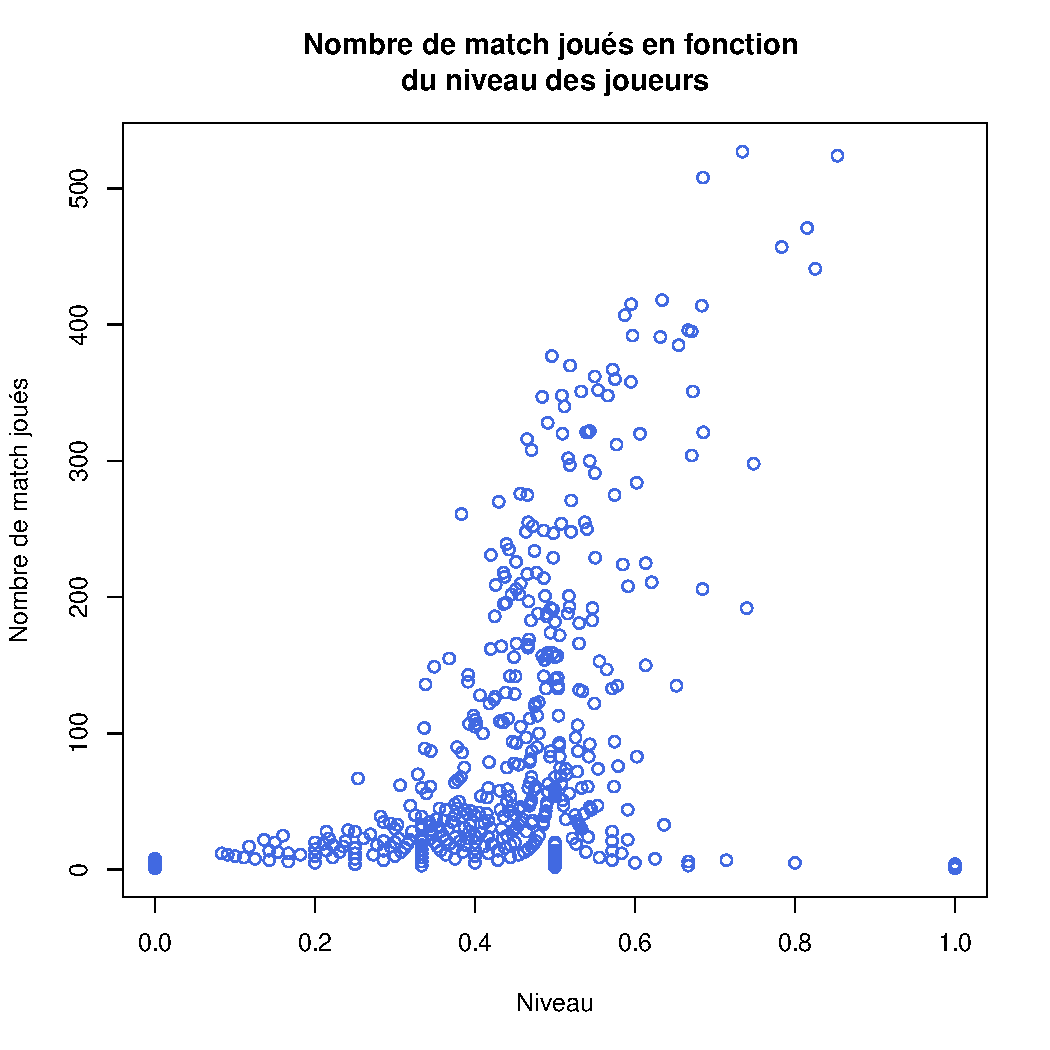
\includegraphics[width=0.35\textwidth]{nb_match_joues_fonction_niveau.pdf}
    \captionof{figure}{Catégorisation du nombre de matchs joués en fonction du niveau des joueurs}\label{fig:tennis1}
\endgroup

Grâce aux données des $26000$ matchs joués, nous avons pu calculer la propension de chaque joueur à gagner un match.
Parmi ces joueurs, seulement $899$ ont au moins gagné un match et $1502$ ont au moins perdu un match ce qui fait que $603$ joueurs n'ont pas gagné de matchs mais ont seulement perdu. Enfin, on a pu remarquer que $66798$ paris, soit 52,82\% de l'ensemble, ont évolué vers le joueur gagnant

De plus, si l’on affiche le nombre de matchs de matchs joués par les joueurs en fonction de leur niveau, on peut observer les points suivants (figure \ref{fig:tennis1}) :

\begin{itemize}

  \item Les joueurs qui possèdent un ratio extrême (proche de $0$ ou de $1$) sont surtout ceux ayant joué peu de matchs, on peut donc ne pas les considérer.
  
  \item La majorité des joueurs a un ratio compris entre $0.4$ et $0.6$ dès qu’un joueur a joué plus de de $100$ matchs.
  
  \item Cependant, après le seuil des $100$ matchs, on observe que les points semblent suivre une tendance linéaire, plus les joueurs ont joués de matchs, plus leur ratio est élevé. On peut expliquer cette tendance par le fait que les joueurs qui on joué un grand nombre de matchs sont sûrement ceux étant restés longtemps dans les tournois (et le circuit) : ils ont certainement un meilleur niveau de part leur longévité au sein du circuit professionnel et du fait qu'ils gagnent des matchs, ce qui semble cohérent.

\end{itemize}

Finalement on pourra noter que pour calculer le niveau nous avons effectuer un ratio entre le nombre de matchs gagnés par le nombre de matchs joués. Nous avons également pensé à faire un niveau en fonction de la moyenne des côtes d'entrées du joueur par match. Plus sa moyenne de côtes est faible, meilleur il est. Mais cela n'aurait pas résolu le problème lié aux joueurs ayant effectué très peu de matchs et répartis avec un niveau proche de $0$ ou $1$. Certes, ils auraient pu avoir un niveau plus réel mais sur un échantillon de $1$ ou $2$ matchs perdus, ce qui est très peu représentatif.


Dans le cadre de notre étude, on considérera comme suspects les matchs dont au moins un des paris présente une évolution de probabilité en valeur absolue strictement supérieure à $0.10$. Ainsi, on remarque qu'il y a $2798$ matchs suspects sur les $25993$ étudiés, ce qui représente environs $10.76$ \% des matchs.

\begingroup
    \centering
   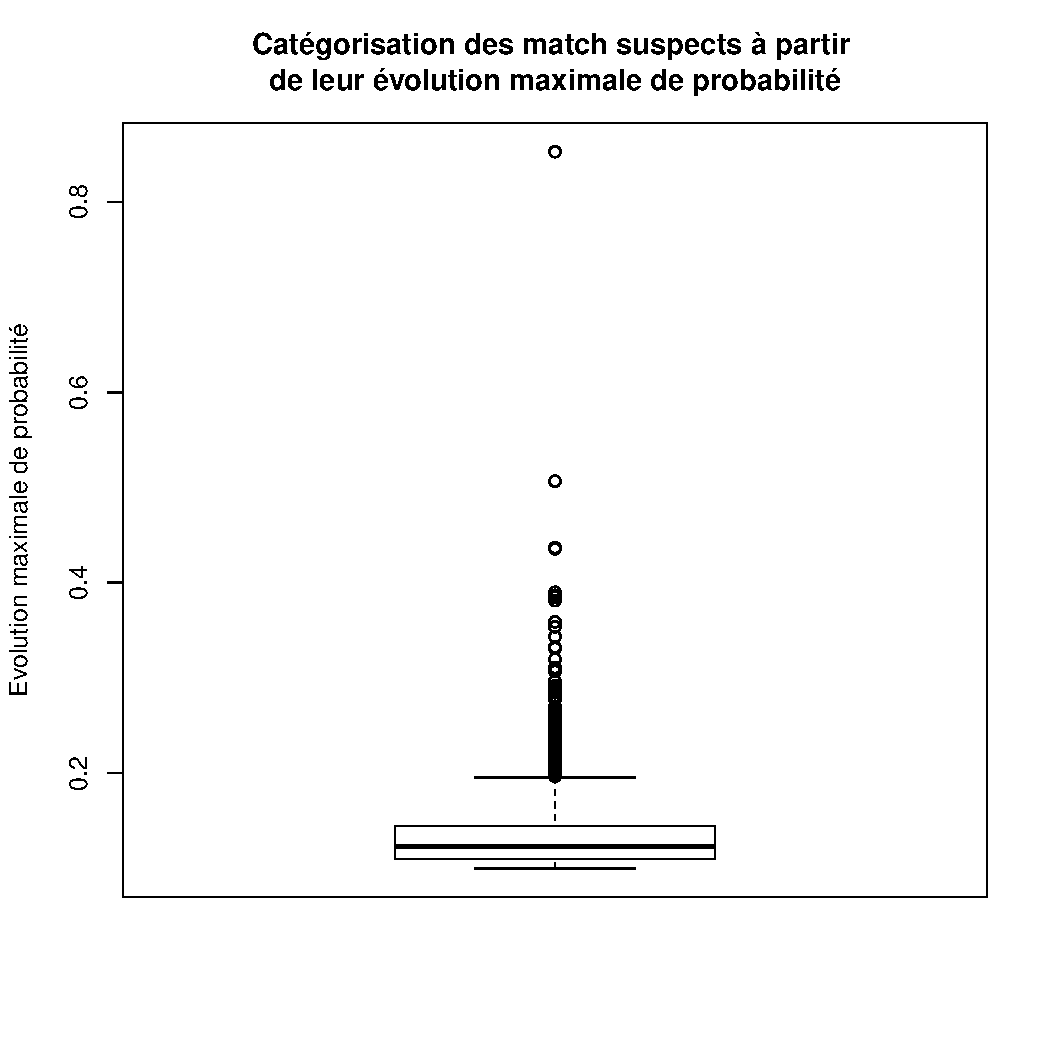
\includegraphics[width=0.35\textwidth]{boxplot_caracterisation_match_suspects_evolution_probabilite.pdf}
    \captionof{figure}{Catégorisation des match suspects à partir de leur évolution maximale de probabilité}\label{fig:tennis2}
\endgroup

On remarque trivialement que plus de $75$ \% des matchs considérés comme suspects ont une évolution maximale de probabilité strictement inférieure à $0.2$  (figure \ref{fig:tennis2}). Tous les outliers ont une évolution maximale de probabilité supérieure à $0.2$. Ainsi, il serait probablement pertinent de s'intéresser particulièrement aux matchs présentant une évolution maximale de probabilité supérieure à $0.2$. Par ailleurs, on notera également que tous les matchs, à l'exception d'un, présentent une évolution maximale de probabilité strictement inférieure à $0.6$. Le match exceptionnel présente une évolution maximale de probabilité de $0.8$, ce qui est particulièrement élevé et donc suspect.

Il s'avère que les $7$ bookmakers ayant effectué des prises de positions sur les $25993$ sont tous impliqués dans des matchs suspects. Dans le diagramme en bâtons représentant le nombre de paris suspects dans lesquels sont impliqués chaque bookmaker (figure \ref{fig:tennis3}), on peut noter que les bookmakers $D$, $E$, $F$ et $G$ sont tous impliqués dans moins de $300$ paris suspects. Cependant, les bookmakers $A$, $B$ et $C$ sont tous impliqués dans plus de $1000$ paris suspects. Il serait dont probablement pertinent de mener une étude plus approfondie sur ces trois derniers bookmakers. 

\begingroup
    \centering
   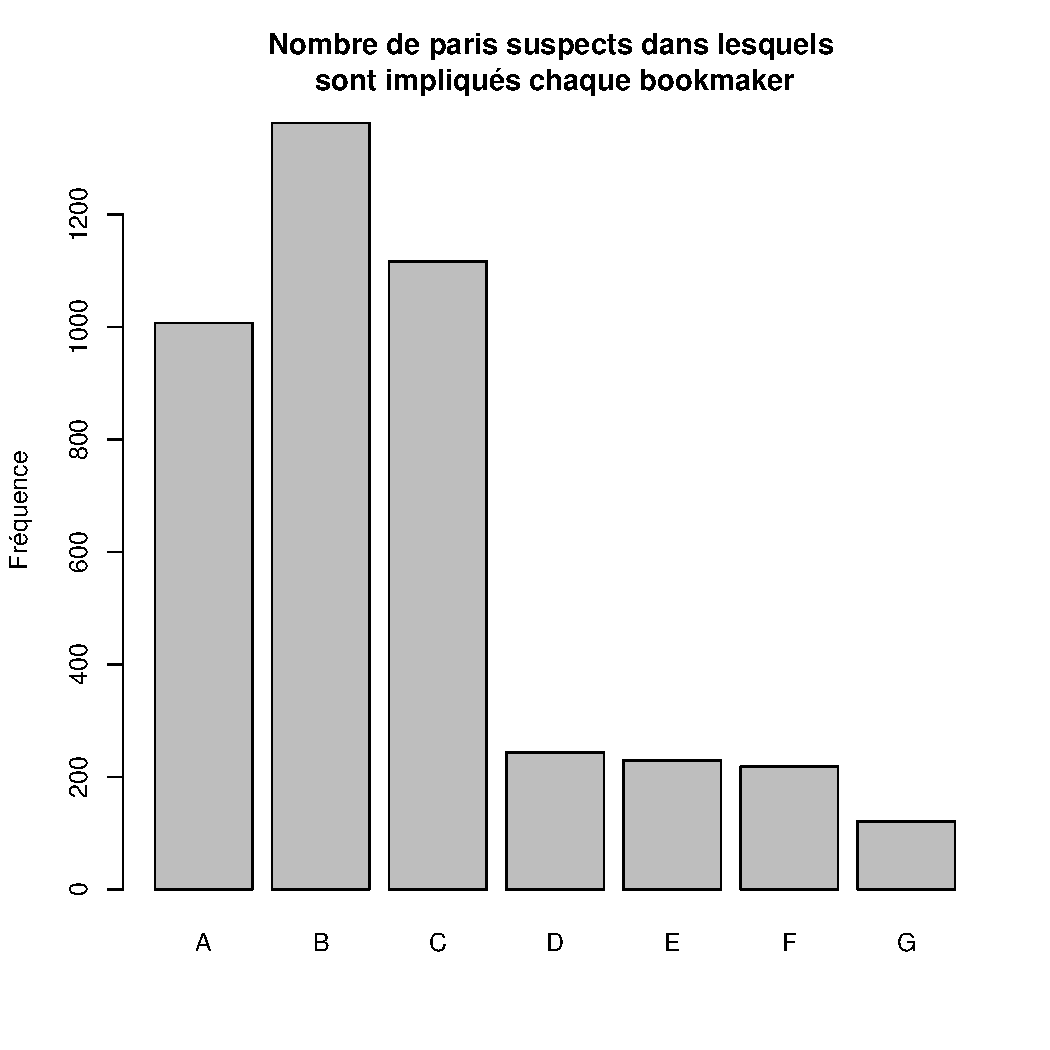
\includegraphics[width=0.35\textwidth]{nb_paris_suspects_par_bookmaker.pdf}
    \captionof{figure}{Nombre de paris suspects dans lesquels sont impliqués chaque bookmaker}\label{fig:tennis3}
\endgroup

Dans notre analyse, on considère que les gagnants suspects sont ceux ayant gagné un match considéré comme suspect. De même, les perdants considérés comme suspects sont ceux ayant perdu un match considéré comme suspect. L'union des gagnants et des perdants suspects forme l'ensemble des joueurs suspects. Il est particulièrement intéressant de constater qu'il y a $559$ perdants suspects, $455$ gagnants suspects et $655$ joueurs suspects. Ainsi, on peut facilement remarquer que $359$ ($359 = (559 + 455) -655 $) des joueurs suspects sont à la fois des gagnants et des perdants suspects. En considérant qu'il est plus simple d'influencer l'issue d'un match en le perdant contre toute attente qu'en le gagnant contre toute attente, nous nous intéresserons plus particulièrement aux perdants suspects. 

\begingroup
    \centering
   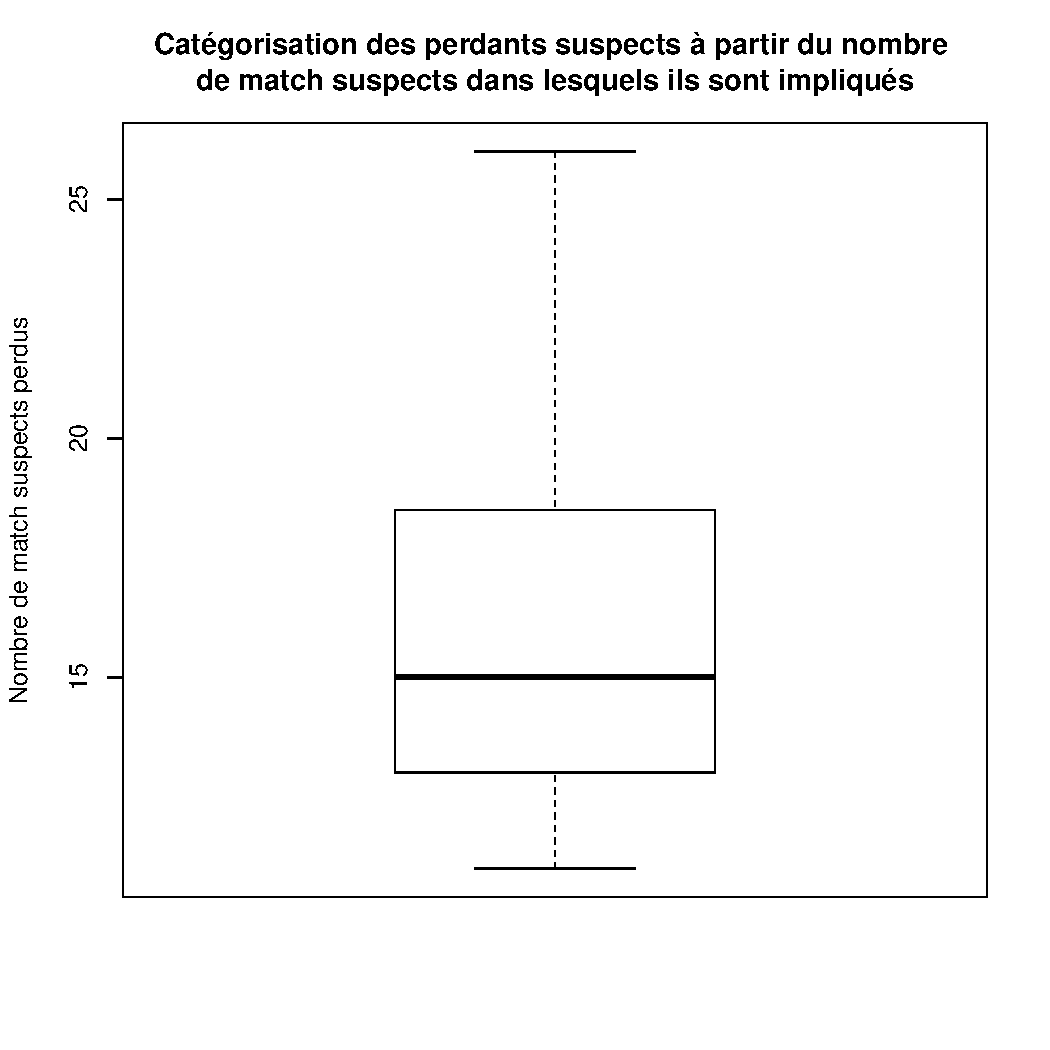
\includegraphics[width=0.35\textwidth]{boxplot_caracterisation_perdants_suspects_nb_match_suspects.pdf}
    \captionof{figure}{Catégorisation des perdants suspects à partir du nombre
de matchs suspects dans lesquels ils sont impliqués}\label{fig:tennis4}
\endgroup

Parmi ces derniers, seuls $87$ ont perdu plus de $10$ matchs considérés comme suspects (on pourra noter qu'il y en a $17$ qui ont perdu exactement $10$ matchs suspects). Plus de $75$ \% de ces $87$ joueurs ont perdu moins de $20$ matchs (figure \ref{fig:tennis4}). Il serait donc particulièrement pertinent de mener une étude plus approfondie sur les autres joueurs (ceux ayant perdu plus de $20$ matchs suspects). 

\subsection{Données crabs}
\label{sub_sec_donnees_crabs}
%Mettre en colonne les graphs (sur 2 colonnes)
Le jeu de données considéré est disponible dans la bibliothèque de fonctions \texttt{MASS}. Il est constitué de $200$ crabes de l'espèce \textit{Leptograpsus variegatus} collectés à Fremantle, en Australie. Ces crabes sont décrits par $8$ variables : $3$ variables qualitatives et $5$ quantitatives.

% \begin{multicols}{2} % Style double colonne 

\begingroup
    \centering
   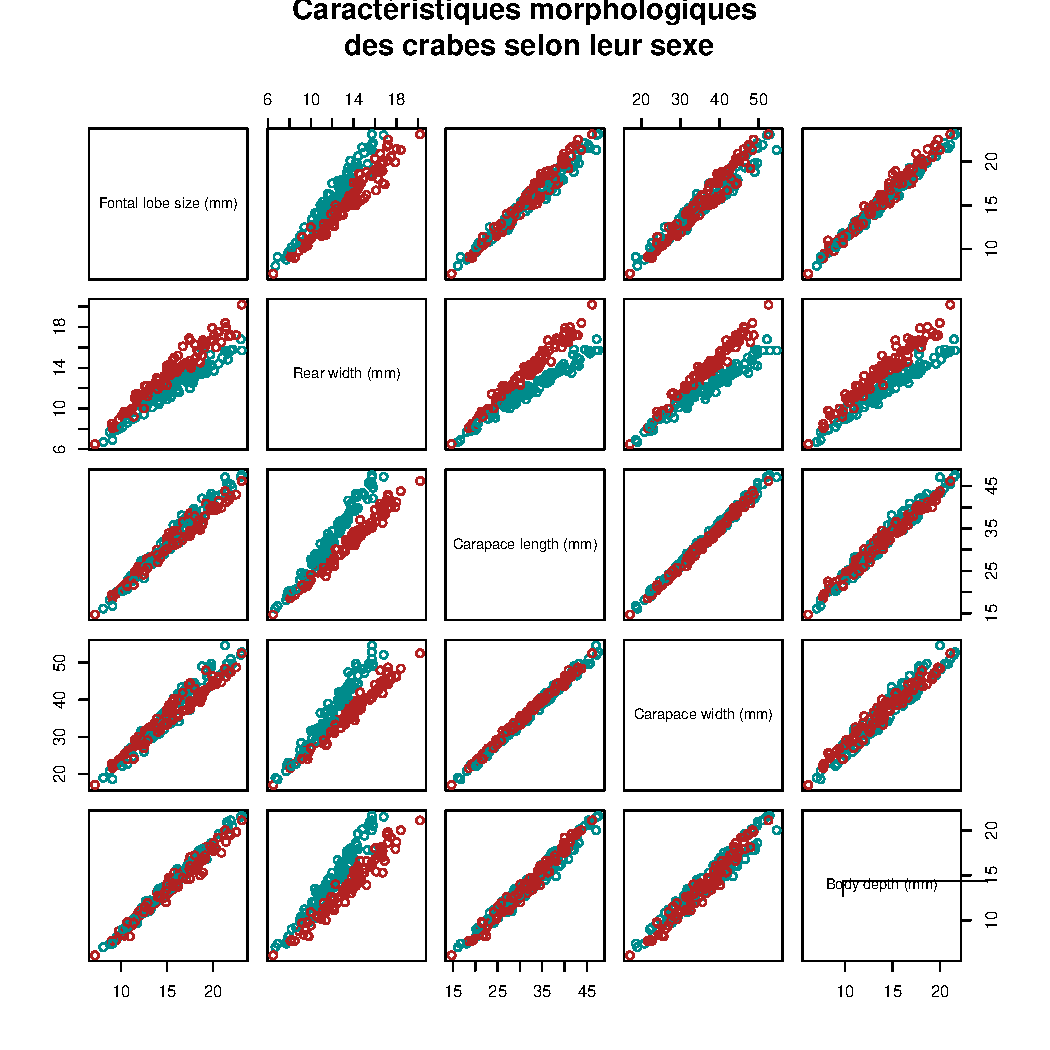
\includegraphics[width=0.35\textwidth]{crabes_selon_sexe.pdf}
    \captionof{figure}{Comparaison des caractéristiques morphologiques des crabes par sexe}\label{fig:crabs121}
\endgroup

\begingroup
    \centering
   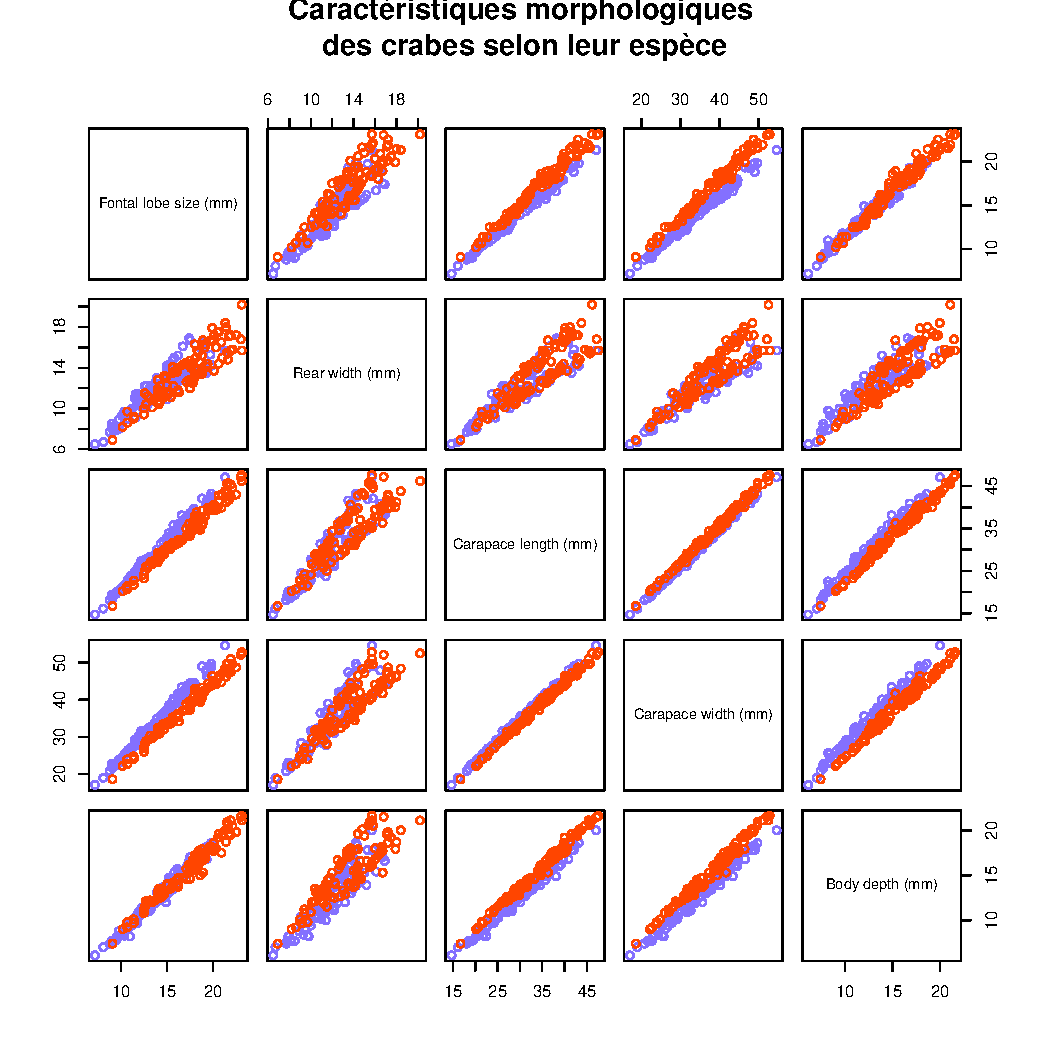
\includegraphics[width=0.35\textwidth]{crabes_selon_espece.pdf}
    \captionof{figure}{Comparaison des caractéristiques morphologiques des crabes par espèce}\label{fig:crabs122}
\endgroup

% \end{multicols}

Tout d'abord, il est particulièrement intéressant de constater que l'échantillon est constitué de $50$ crabes mâles et bleu, $50$ crabes mâles et orange, $50$ crabes femelles et bleu ainsi que de $50$ crabes femelles et orange. Ainsi, chacune des quatre variétés de crabes est autant représentée que les autres.   

% \begin{multicols}{2}

\begingroup
    \centering
   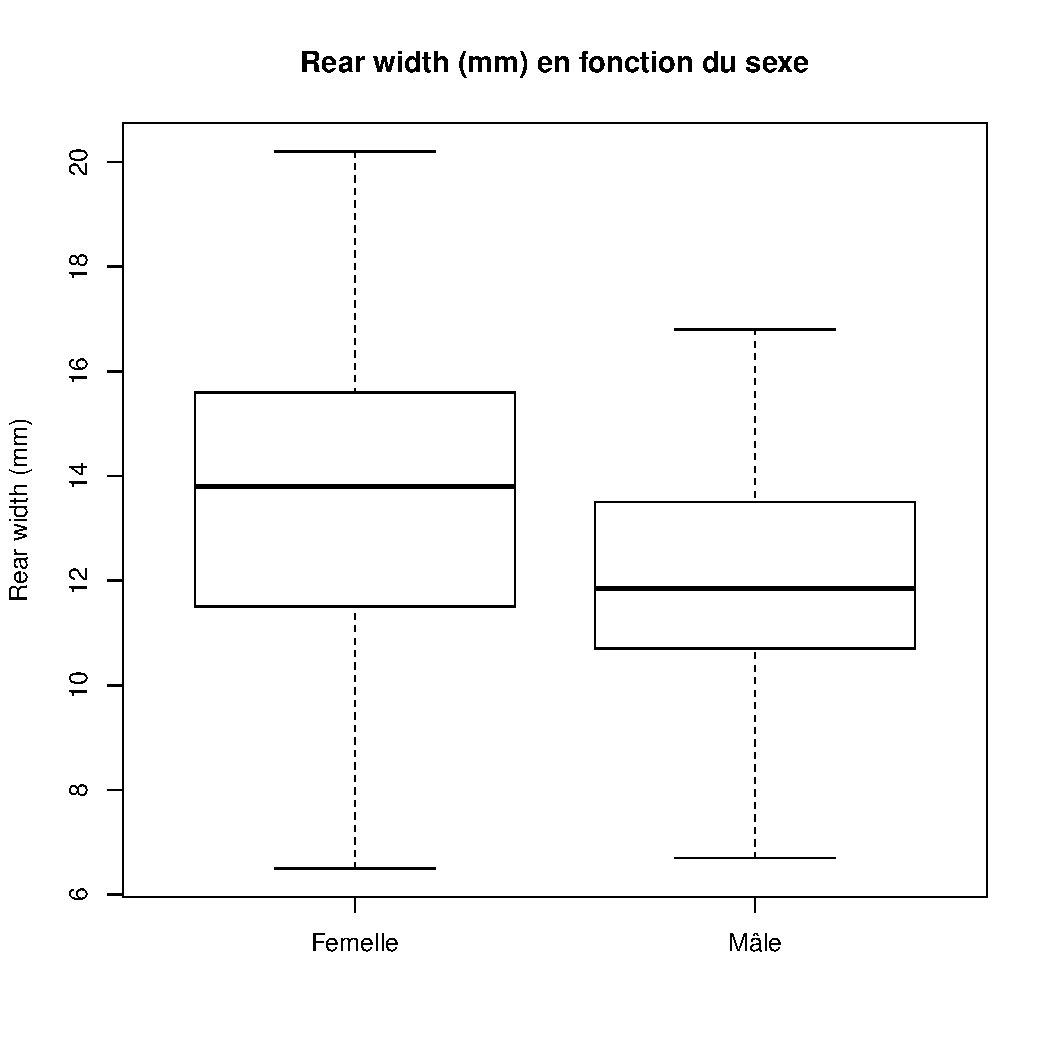
\includegraphics[width=0.35\textwidth]{boxplot_rear_width_fonction_sexe.pdf}
    \captionof{figure}{Boxplot rear width (mm) en fonction du sexe}\label{fig:crabs123}
\endgroup

\begingroup
    \centering
   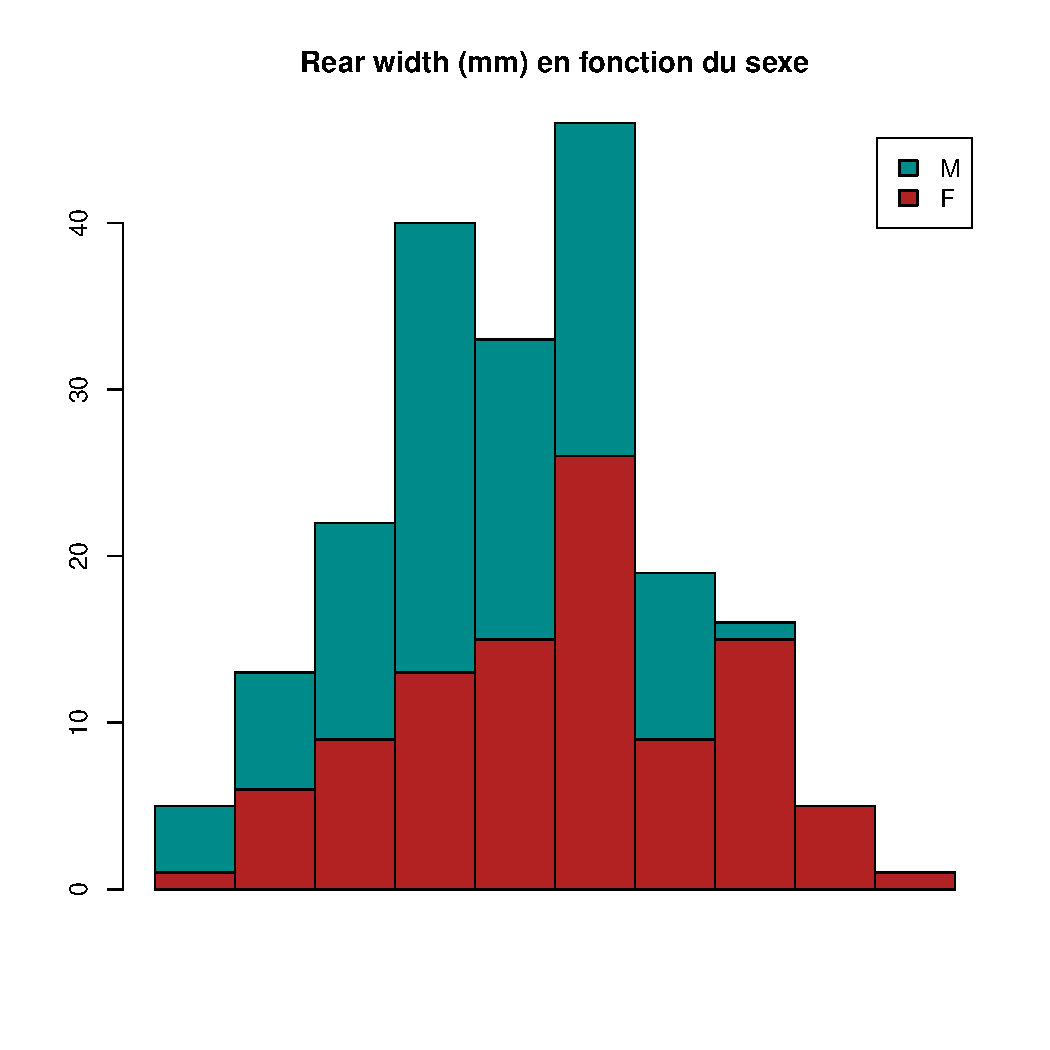
\includegraphics[width=0.35\textwidth]{hist_rear_width_fonction_sexe.pdf}
    \captionof{figure}{Barplot rear width (mm) en fonction du sexe}\label{fig:crabs124}
\endgroup

% \end{multicols}

En représentant les individus de l'échantillon selon leur sexe, tour à tour, en fonction de $2$ variables quantitatives parmi les $5$ à notre disposition (figure \ref{fig:crabs121}), il semblerait que le paramètre \texttt{Rear width} soit impacté par le sexe de l'individu. Afin de mieux observer ce phénomène, nous avons tenté de catégoriser les individus de la population selon leur sexe et leur réalisation pour le paramètre \texttt{Rear width}. Via les deux diagrammes en boîte consultables dans la figure \ref{fig:crabs123}, on constate que près de $50$ \% des femelles possèdent plus de $14$ pour le paramètre \texttt{Rear width} tandis que plus de $75$ \% des mâles ont moins de $14$ pour le même paramètre. Ainsi, notre hypothèse semble être confortée par ces deux diagrammes (figures \ref{fig:crabs123} et \ref{fig:crabs124}).

% \begin{multicols}{2}

\begingroup
    \centering
   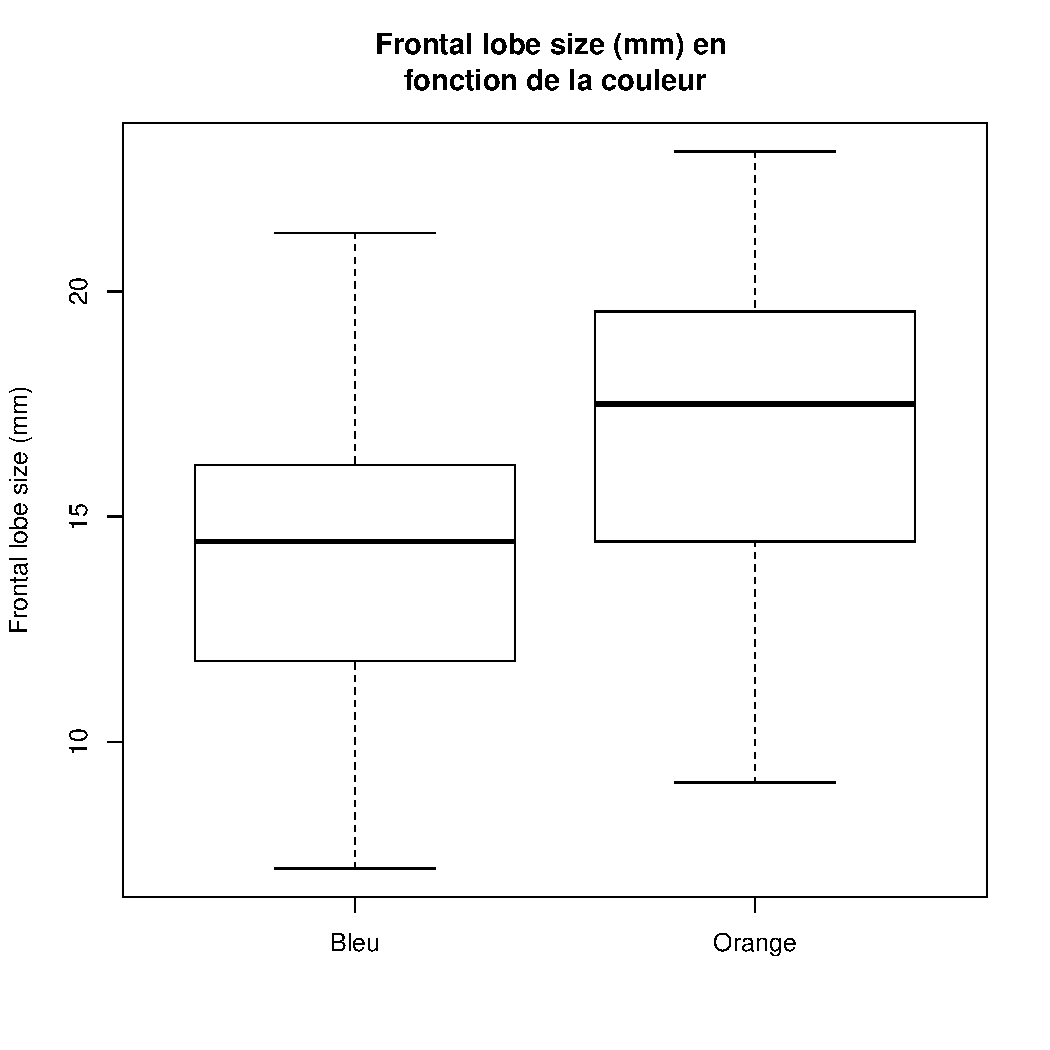
\includegraphics[width=0.35\textwidth]{boxplot_frontal_lobe_size_fonction_espece.pdf}
    \captionof{figure}{Boxplot frontal lobe size (mm) en fonction de la couleur}\label{fig:crabs125}
\endgroup

\begingroup
    \centering
   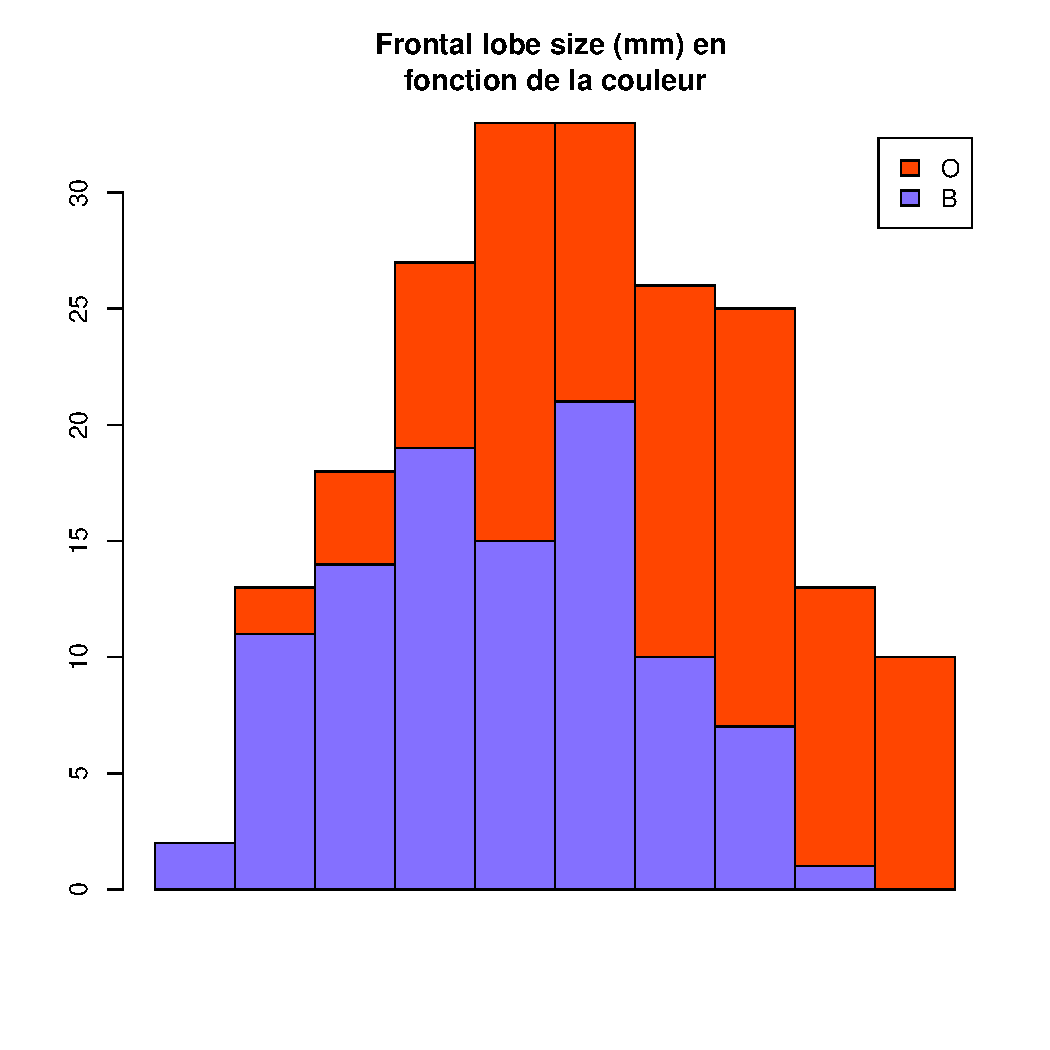
\includegraphics[width=0.35\textwidth]{hist_frontal_lobe_size_fonction_espece.pdf}
    \captionof{figure}{Barplot frontal lobe size (mm) en
fonction de la couleur}\label{fig:crabs126}
\endgroup

% \end{multicols}

De la même manière, en représentant les individus de l'échantillon selon leur couleur, tour à tour, en fonction de $2$ variables quantitatives parmi les $5$ à notre disposition (figure \ref{fig:crabs122}), il semblerait que les paramètres \texttt{Frontal lobe size} et \texttt{Carapace width} soient impactés par la couleur de l'individu. Afin de mieux observer ce phénomène pour le paramètre \texttt{Frontal lobe size}, nous avons tenté de catégoriser les individus de la population selon leur couleur et leur réalisation pour le paramètre \texttt{Frontal lobe size}. Via les deux diagrammes en boîte consultables dans la figure \ref{fig:crabs125}, on constate que près de $75$ \% des crabes orange possèdent plus de $15$ pour le paramètre \texttt{Fontal lobe size} tandis que plus de $50$ \% ont moins de $15$ pour le même paramètre. Ainsi, notre hypothèse semble être confortée par ces deux diagrammes (figures \ref{fig:crabs125} et \ref{fig:crabs126}).

En visualisant les graphiques de dispersion de tous les couples de variables présents dans les figures \ref{fig:crabs121} et \ref{fig:crabs122}, il semblerait que les points représentant les individus de notre échantillon se regroupent autour de droites. Ainsi, on peut logiquement penser qu'il y a des relations linéaires entre chaque couple de variables. Afin de vérifier cela, nous avons calculé la matrice des corrélations $R$ (table \ref{tab_correlations}) associée à la matrice liée au tableau individus-variables. Il s'avère que chacun des éléments de cette matrice a une valeur strictement supérieure à $0.85$ :  ce phénomène semble conforter notre hypothèse.  

\begin{table}[H]
  \begin{center}
  \resizebox{\columnwidth}{!}{%
  \begin{tabular}{|c||c|c|c|c|c|}
   \hline			
     \diagbox{}{} & FL & RW & CL & CW & BD \\
   \hline
   \hline
     FL & $1.0000000$ & $0.9069876$ & $0.9788418$ & $0.9649558$ & $0.9876272$\\
   \hline
     RW & $0.9069876$ & $1.0000000$ & $0.8927430$ & $0.9004021$ & $0.8892054$\\
   \hline
     CL & $0.9788418$ & $0.8927430$ & $1.0000000$ & $0.9950225$ & $0.9832038$\\
   \hline
     CW & $0.9649558$ & $0.9004021$ & $0.9950225$ & $1.0000000$ & $0.9678117$\\
    \hline
     BD & $0.9876272$ & $0.8892054$ & $0.9832038$ & $0.9678117$ & $1.0000000$\\
  \hline  
  \end{tabular}
  }
  \end{center}
  \caption{La matrice de corrélation}
  \label{tab_correlations}
\end{table}

Afin d'illustrer nos dires, par ailleurs, nous avons mené un test de corrélation de Pearson entre les variables \texttt{Carapace length (mm)} et \texttt{Carapace width (mm)}. 

\begingroup
    \centering
   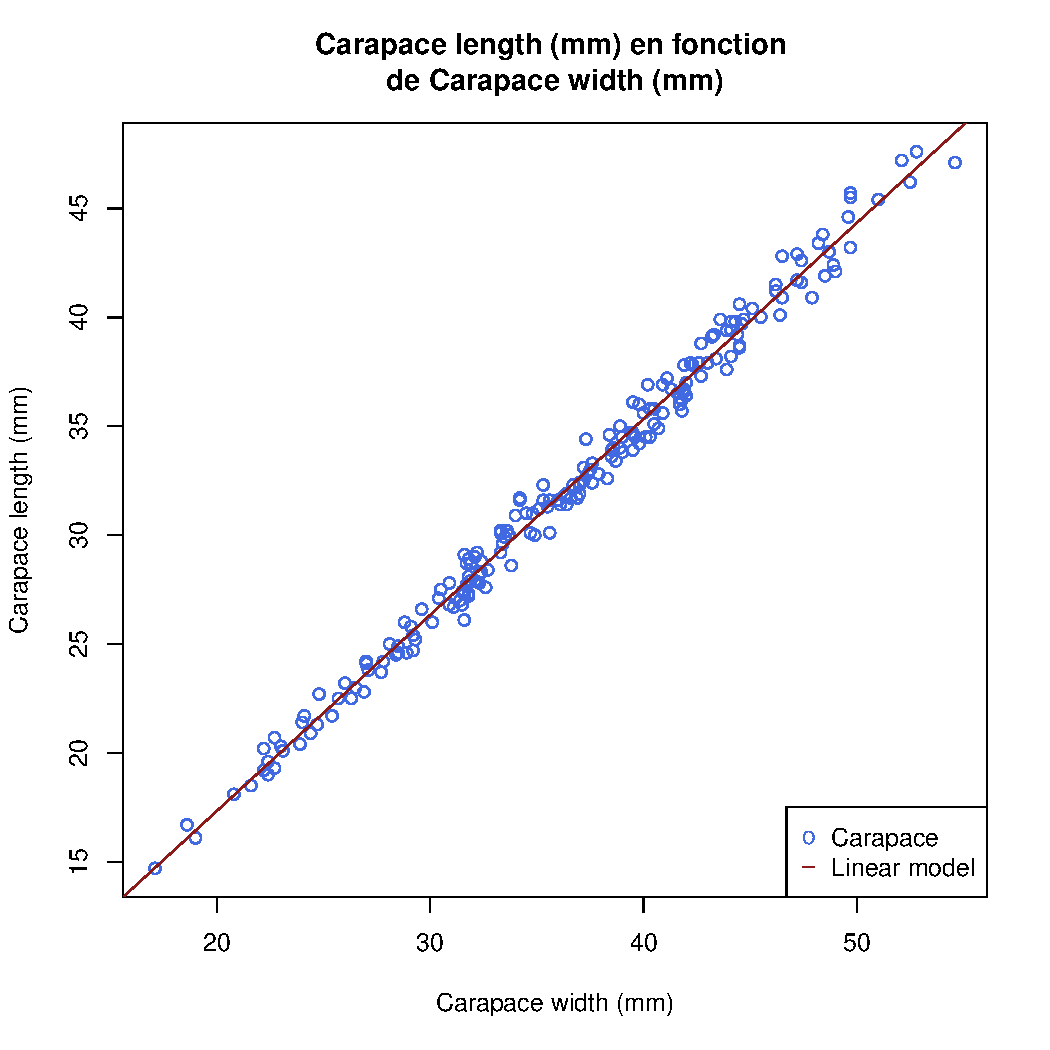
\includegraphics[width=0.35\textwidth]{carapace_length_fonction_carapace_width.pdf}
    \captionof{figure}{Carapace length (mm) en fonction de Carapace width (mm)}\label{fig:crabs127}
\endgroup

Nous nous sommes permis d'utiliser ce test car nous jugeons que les réalisations de ces deux paramètres semblent être issues de variables aléatoires parentes de loi Gaussienne. De plus, d'après les figures \ref{fig:crabs121} et \ref{fig:crabs122}, il y a absence de valeurs exceptionnelles pour les réalisations de ces deux variables. L'hypothèse nulle de ce test, notée $H_0$, est que le coefficient de corrélation entre ces deux variables est de $0$, soit qu'il y ait absence de corrélation entre ces deux variables. Pour ce test, nous nous sommes fixés comme seuil de signification $\alpha^{\ast} = 0.01$. Cela signifie que l'on s'autorise à commettre une erreur de première espèce $\alpha$ inférieure à $0.01$ (probabilité de rejeter l'hypothèse nulle $H_0$ sachant que cette dernière est vraie). Après avoir effectué le test, il s'avère que l'on retrouve le coefficient de corrélation $0.9950225$ précédemment trouvé. Par ailleurs, l'intervalle de confiance pour ce coefficient de corrélation au niveau $1-\alpha = 0.95$ est : $[0.9934242, 0.9962331]$. On remarque que cet intervalle est particulièrement petit pour un niveau de confiance si élevé, cela conforte à nouveau notre intuition. La valeur p (p-value) est strictement inférieure à $2.2^{-16}$. Autrement dit, nous rejetons $H_0$ puisque cette dernière est inférieure à notre seuil de signification $\alpha^{\ast}$. Ainsi, il y a donc a priori présence d'une relation linéaire entre les paramètres \texttt{Carapace length (mm)} et \texttt{Carapace width (mm)}. Afin d'exhiber ce phénomène, nous avons également réalisé une régression linéaire entre ces deux paramètres. Après calcul, on obtient une ordonnée à l'origine de $b = -0.6619$ et une pente de $a = 0.8998$.  Le résultat associée à la régression linéaire est consultable dans la figure \ref{fig:crabs127}. Ce phénomène est particulièrement intéressant puisque en ayant recours à l'équation \ref{eq_linear_reg}, en connaissance de \texttt{CW} (\texttt{Carapace width (mm)}), on peut prédire \texttt{CL} (\texttt{Carapace length (mm)}) et réciproquement. 

\begin{equation}
  \label{eq_linear_reg}
  CL = a * CW + b = 0.8998 * CW -0.6619
\end{equation}

\section{Analyse en composantes principales}

\subsection{Exercice théorique}

Trois variables mesurées sur quatre individus forment la matrice $Y$ présente dans l'équation \ref{eq_theoric_data}.

\begin{equation}
	\label{eq_theoric_data}
    Y = 
    \begin{pmatrix}
      3 & 4 & 3 \\
      1 & 4 & 3 \\
      2 & 3 & 6 \\
      4 & 1 & 2   
    \end{pmatrix}
\end{equation}

Afin de calculer, les axes factoriels de l'\texttt{ACP}, nous nous sommes contentés de calculer la matrice de variance $V = X^T D_p X = \frac{1}{n}X^T I_n X$ associée à $X$, $X$ étant la matrice $Y$ ayant subi un centrage, $Y$ étant la matrice initiale des données. A l'issue de ce calcul, nous avons calculé les valeurs propres $\lambda_1, \cdots, \lambda_p$ et leurs vecteurs propres normalisés associés $U = (U_1, \cdots, U_p)$ (ces données sont triées selon les valeurs propres dans l'ordre décroissant). Les axes factoriels correspondent aux vecteurs propres $U_1, \cdots, U_p$ de la matrice $V$.

Pour le calcul du pourcentage d'inertie expliquée $E_{a_i}$ par l'axe $i$, où $i \in [[1, p]]$, nous nous sommes contentés d'appliquer la formule présente dans l'équation \ref{eq_pourcentage_inertie_axe}. Le résultat obtenue est consultable dans la figure \ref{fig:screeplots}.

\begingroup
    \centering
   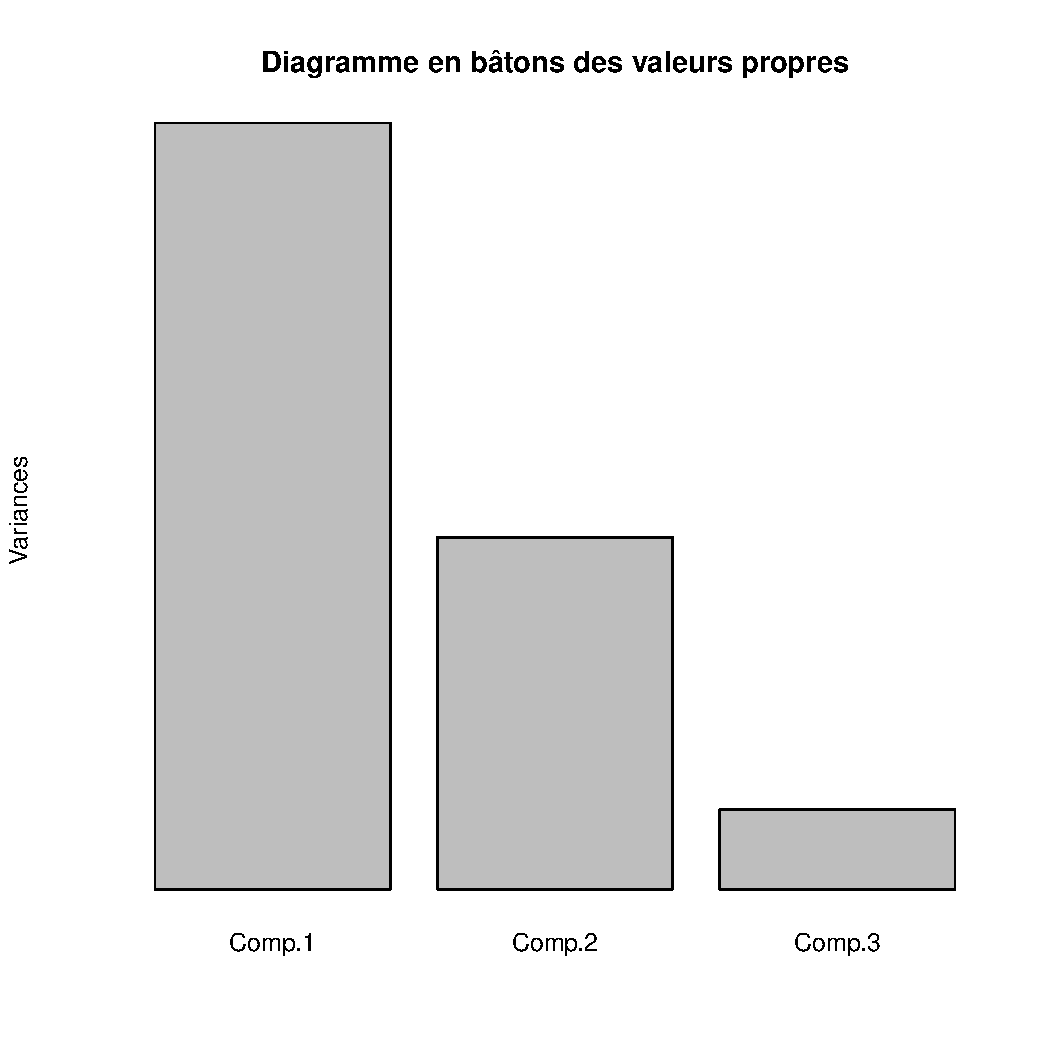
\includegraphics[width=0.35\textwidth]{2_1_barplot_eigenvalues.pdf}
    \captionof{figure}{Scree plot des valeurs propres}\label{fig:screeplots}
\endgroup

\begin{equation}
\label{eq_pourcentage_inertie_axe}
E_{a_i} = 100 \frac{\lambda_i}{\sum_{k = 1}^{p} \lambda_k}
\end{equation}


Pour le calcul des composantes principales $C = (C_1, \cdots, C_p)$, il suffit d'appliquer la formule présente dans l'équation \ref{eq_composantes_principales}.

\begin{equation}
  \label{eq_composantes_principales}
  C = X M U = X I_p U 
\end{equation}

% \begin{multicols}{2}

\begingroup
    \centering
   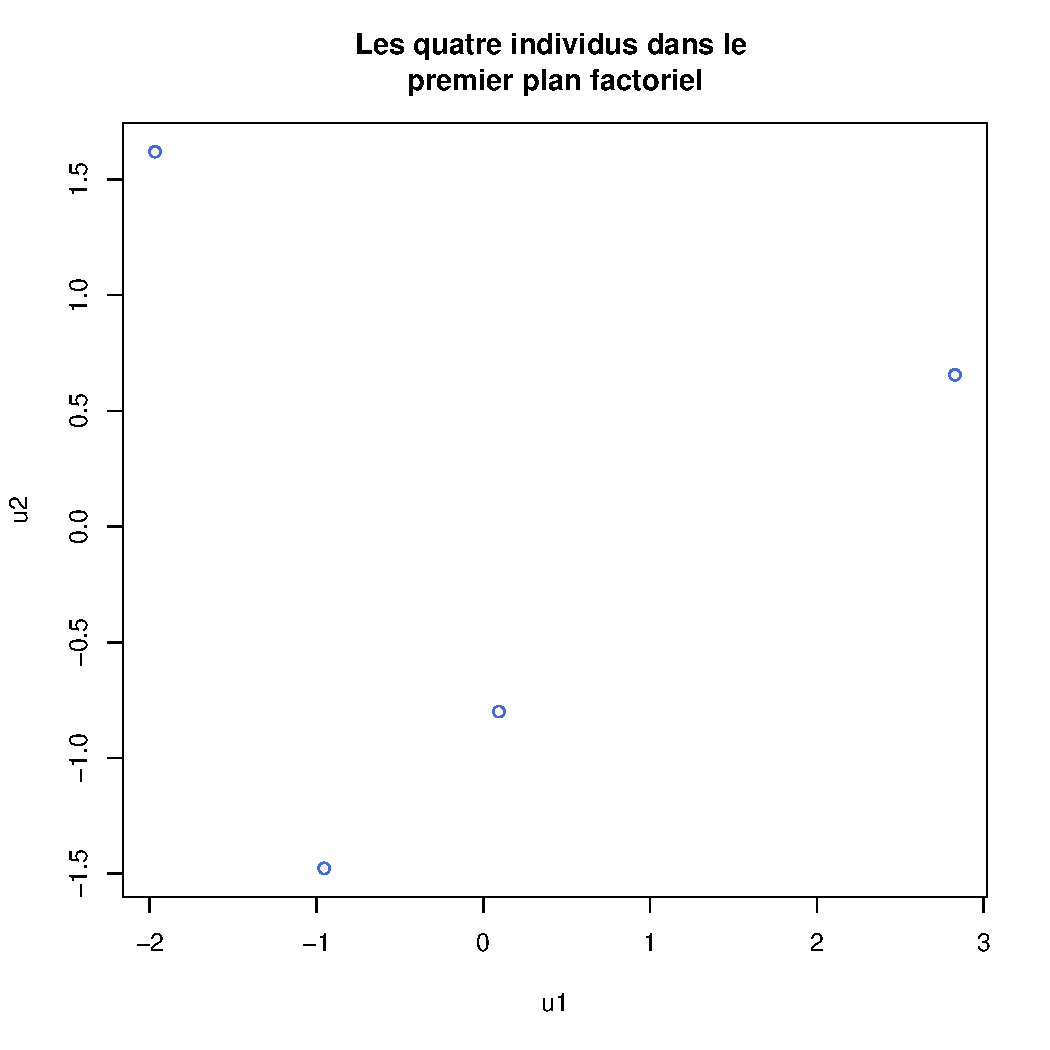
\includegraphics[width=0.35\textwidth]{individus_premier_plan_factorial.pdf}
    \captionof{figure}{Les quatre individus dans le premier plan factoriel}\label{fig:ana211}
\endgroup

\begingroup
    \centering
   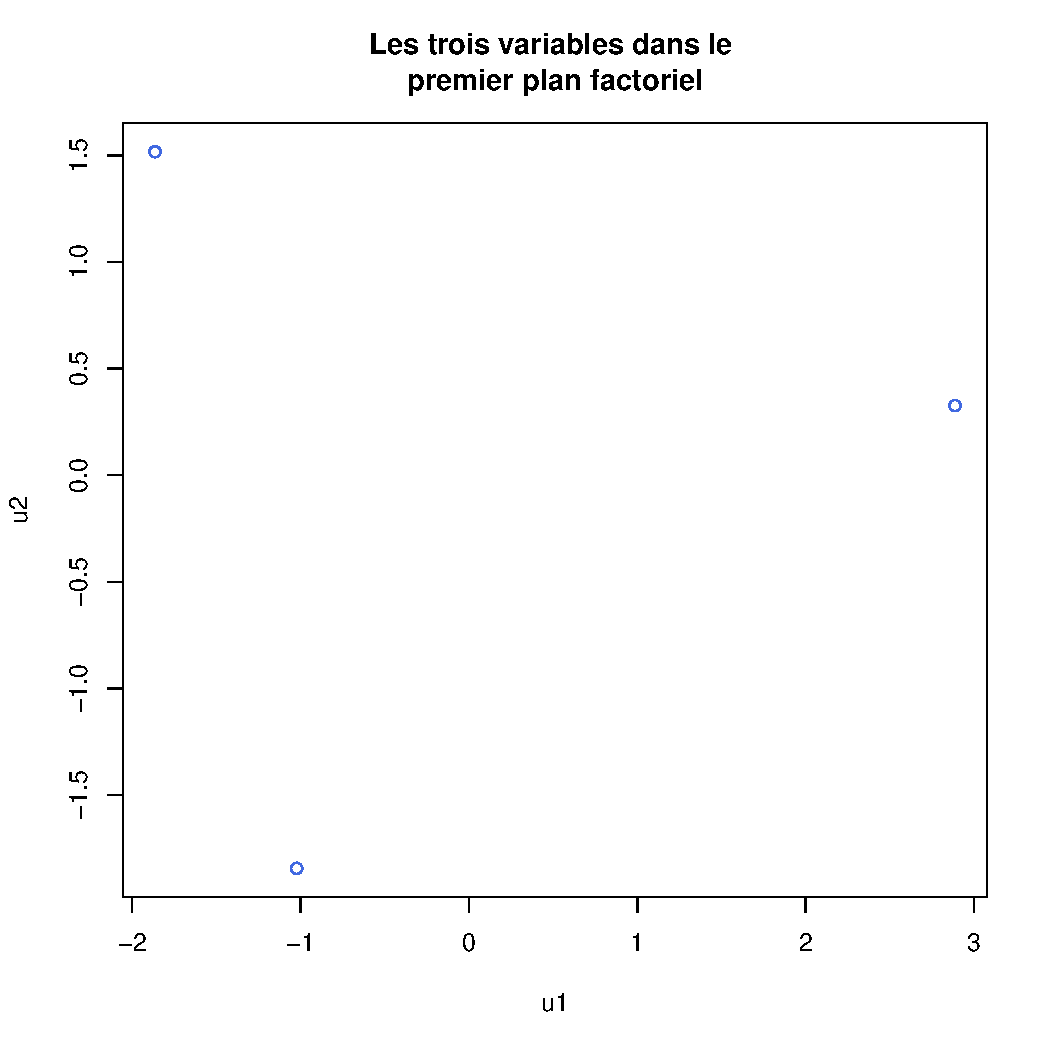
\includegraphics[width=0.35\textwidth]{variables_premier_plan_factorial.pdf}
    \captionof{figure}{Les trois variables dans le premier plan factoriel}\label{fig:ana212}
\endgroup

% \end{multicols}

Pour la représentation des quatre individus dans le premier plan factoriel, il suffit de ne représenter que les données associées aux deux premières colonnes de la matrice $C$ ($C_1$ et $C_2$). Le résultat obtenu est consultable dans la figure \ref{fig:ana211}.

Pour la représentation des trois variables dans le premier plan factoriel, il faut effectuer les même calculs que pour la représentation des quatre individus en n'oubliant pas d'effectuer ces derniers sur la transposée de $Y$. Le résultat obtenu est consultable dans la figure \ref{fig:ana212}.

Nous savons que $X M = C U^T$. Ainsi, on peut en déduire les résultats figurant dans l'équation \ref{eq_reconstitution}.

\begin{equation}
	\label{eq_reconstitution}
    X M = X = C U^T = \sum_{\alpha = 1}^{p} c_{\alpha} u_{\alpha}^T 
\end{equation}

Ainsi, on peut se permettre de calculer l'expression $\sum_{\alpha = 1}^{k} c_{\alpha} u_{\alpha}^T $, pour $k = 1, 2$ et $3$. Lorsque $k=1$, on retrouve les coordonnées dans la base initiale des individus projetés dans le sous espace vectoriel $E_1$ de dimension $1$. De même, lorsque $k=2$, on retrouve les coordonnées dans la base initiale des individus projetés dans le sous espace vectoriel $E_2$ de dimension $2$. Enfin, lorsque $k=3$, on retrouve les coordonnées dans la base initiale des individus projetés dans le sous espace vectoriel $E_3$ de dimension $3$, soit on retrouve la matrice centrée $X$.  

\subsection{Utilisation des outils R}
Dans cette sous-section, on utilise les fonctions \texttt{R} afin d'effectuer l'\texttt{ACP} d'un jeu de données portant sur des notes.

Pour ce faire, comme dans l'exercice précédent, on commence par calculer la matrice des données centrées. Puis, on calcule la matrice $V$ de covariance ainsi que les vecteurs propres et les valeurs propres lui étant associés. Ensuite, on calcule la matrice des composantes principales $C$. On cherche également à obtenir les contributions des axes aux individus et des individus aux axes. Enfin, on représente les variables dans la base des composantes principales. 

\begingroup
    \centering
   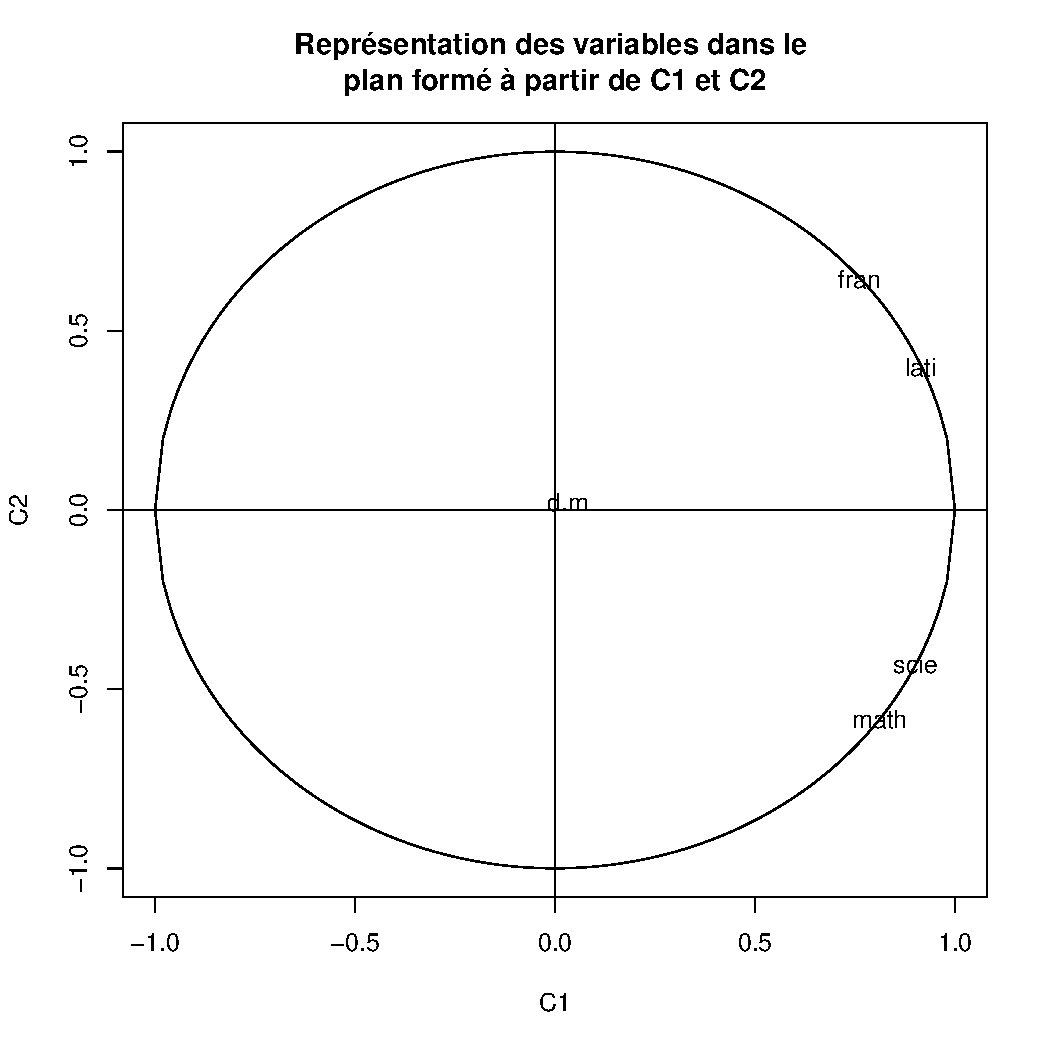
\includegraphics[width=0.35\textwidth]{22variables_c1_c2.pdf}
    \captionof{figure}{Représentation des variables dans le plan formé à partir de C1 et C2}\label{fig:ana221}
\endgroup

Nous avons représenté les $5$ variables dans le plan formé à partir deux premières composantes principales ($C_1$ et $C_2$). Dans la figure \ref{fig:ana221}, on constate que $C_1$ et $C_2$ résument les $4$ premières variables (\texttt{fran}, \texttt{lati}, \texttt{scie} et \texttt{math}). Cependant, $C_1$ et $C_2$ ne donnent pas d'information sur la dernière variable (\texttt{d.m}).

\begingroup
    \centering
   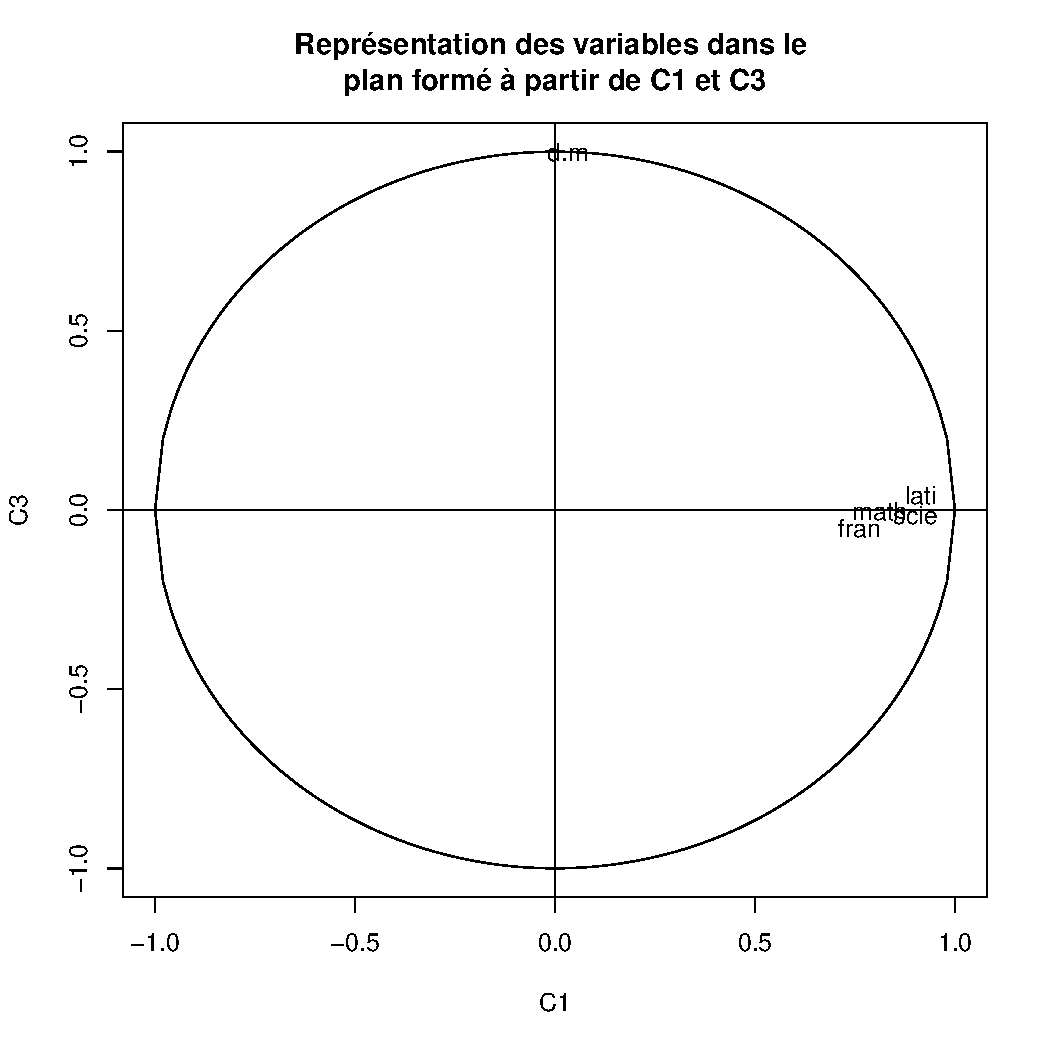
\includegraphics[width=0.35\textwidth]{22variables_c1_c3.pdf}
    \captionof{figure}{Représentation des variables dans le plan formé à partir de C1 et C3}\label{fig:ana222}
\endgroup

De plus, nous avons représenté les variables dans le plan formé à partir de la première et de la troisième composantes principales ($C_1$ et $C_3$). Dans la figure \ref{fig:ana222}, on peut remarquer $C_3$ résume les $4$ premières variables (\texttt{fran}, \texttt{lati}, \texttt{scie} et \texttt{math}) et que $C_1$ représente la dernière variable (\texttt{d.m}).

\begingroup
    \centering
   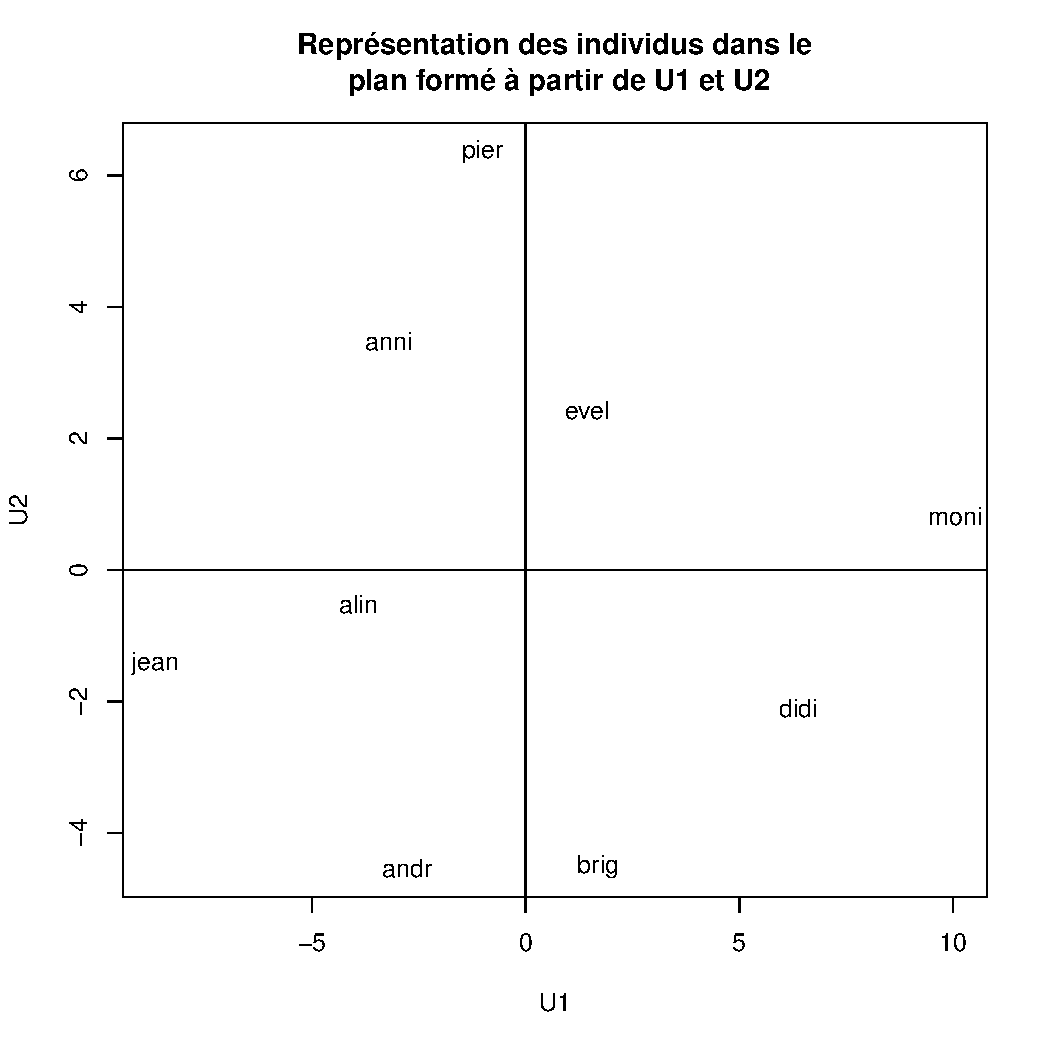
\includegraphics[width=0.35\textwidth]{22individus_u1_u2.pdf}
    \captionof{figure}{Représentation des individus dans le plan formé à partir de U1 et U2}\label{fig:ana223}
\endgroup

Par ailleurs, on a décidé de représenter dans la figure \ref{fig:ana223} les individus dans le plan formé des deux premiers axes factoriels ($U_1$ et $U_2$). Ce graphique souligne le fait que \texttt{jean}, \texttt{alin} et \texttt{andr} ont des notes peu élevées dans les $4$ premières matières (\texttt{fran}, \texttt{lati}, \texttt{scie} et \texttt{math}).

\begingroup
    \centering
   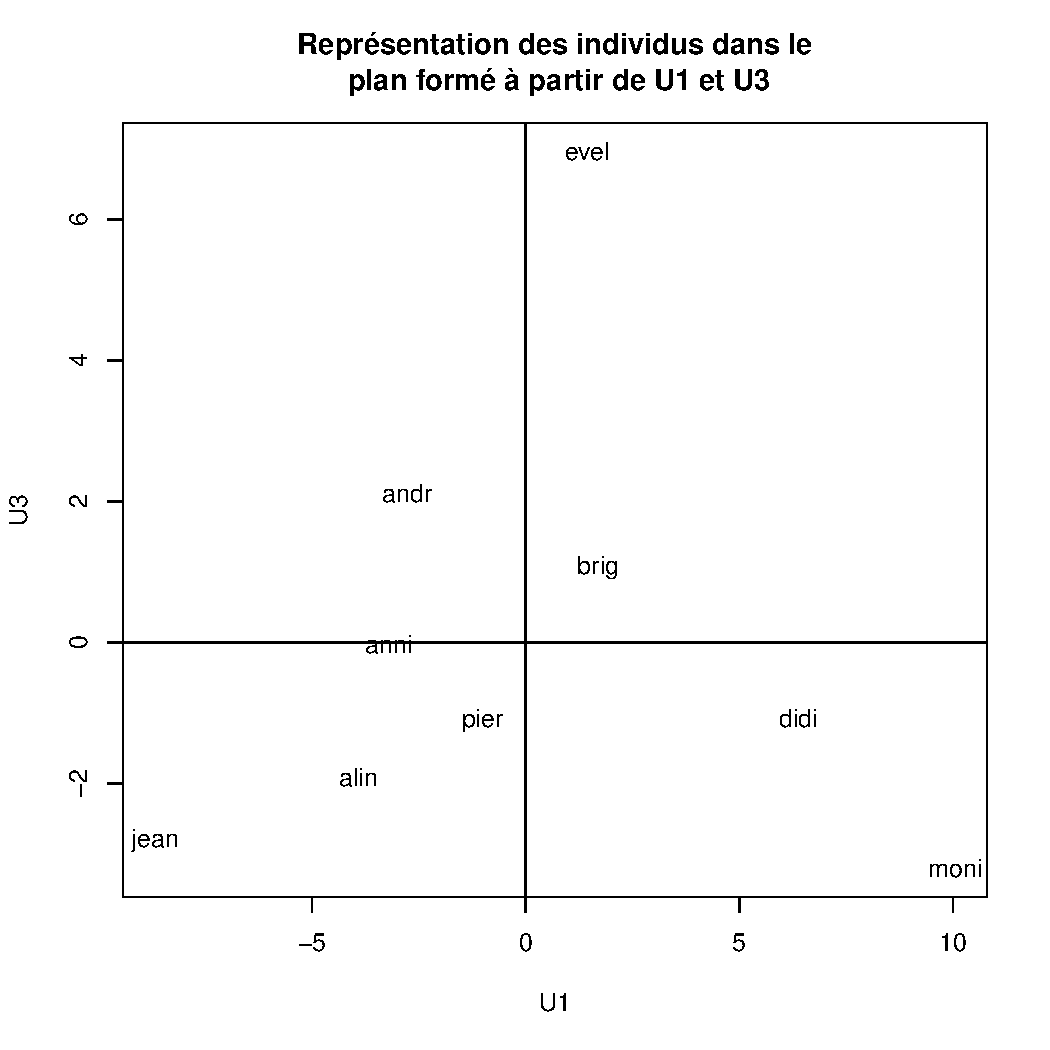
\includegraphics[width=0.35\textwidth]{22individus_u1_u3.pdf}
    \captionof{figure}{Représentation des individus dans le plan formé à partir de U1 et U3}\label{fig:ana224}
\endgroup

De plus, on a décidé de représenter les individus dans le plan formé du premier et du troisième axes factoriels (figure \ref{fig:ana224}). On constate à nouveau que \texttt{jean}, \texttt{alin} et \texttt{andr} ont des notes peu élevées dans les $4$ premières matières. De plus, on note également que \texttt{anni} est dans le même cas. Enfin, on observe que \texttt{evel} a une note très élevée en (\texttt{d.m}). On remarque également que \texttt{moni} est très douée dans les $4$ premières matières mais beaucoup moins en (\texttt{d.m}).

La fonction \texttt{princomp} de \texttt{R} effectue une \texttt{ACP} sur la matrice des données lui étant envoyée en paramètre et renvoie les résultats dans un objet de la classe \texttt{princomp}.

L'attribut \texttt{sdev} de l'objet retourné contient l'écart-type de chaque composante principale. En élevant au carré cet attribut (cela revient à calculer la variance de chaque composante principale), on retrouve logiquement les valeurs propres de la matrice de covariance $V$.

Sur l'objet retourné, la fonction \texttt{plot} affiche un diagramme en bâtons des valeurs propres (scree plot). Cela permet de trouver visuellement et simplement les composantes principales principalement responsables de la dispersion dans les données \ref{fig:ana227}.

\begingroup
    \centering
   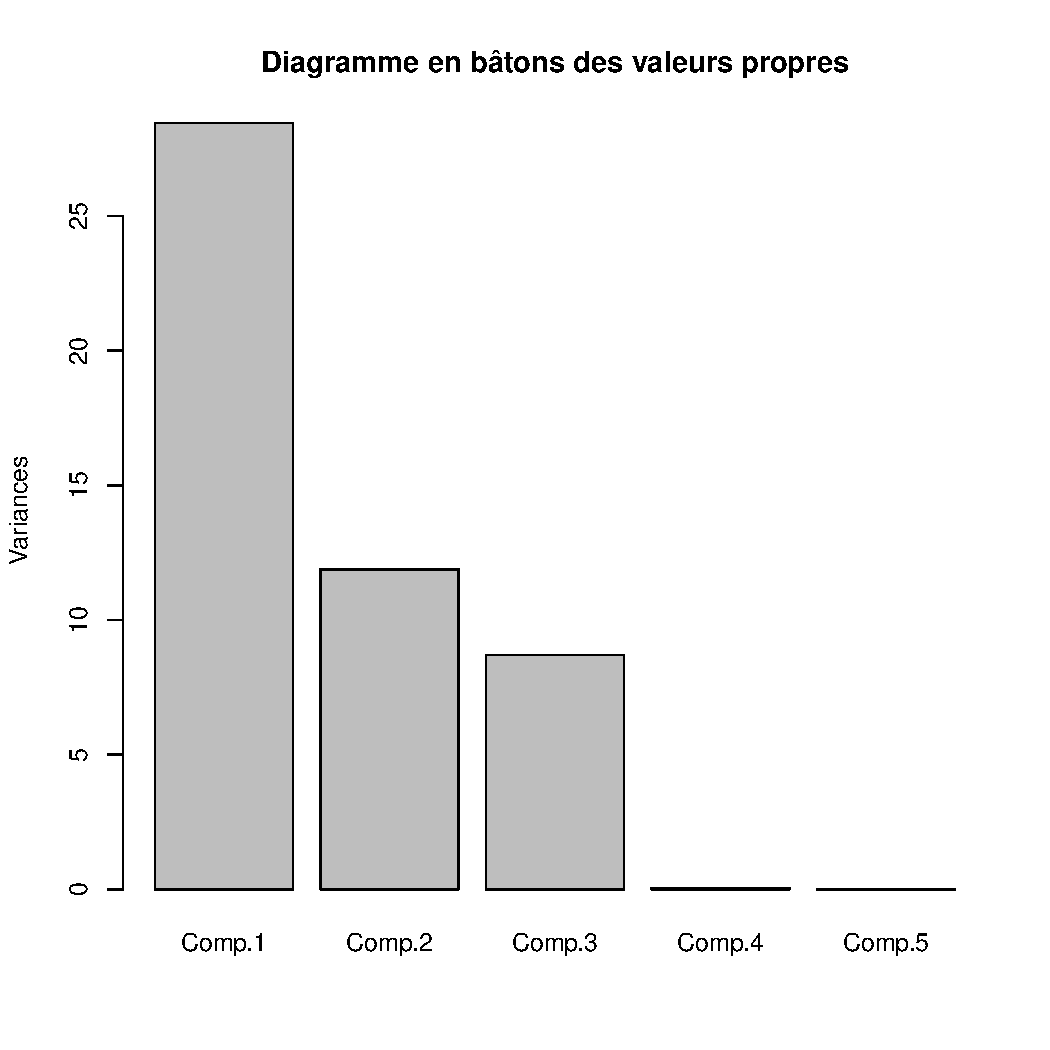
\includegraphics[width=0.35\textwidth]{22batons_valeurs_propres.pdf}
    \captionof{figure}{Scree plot des valeurs propres}\label{fig:ana227}
\endgroup

La fonction \texttt{biplot} permet de représenter les individus et les variables sur le même graphique. Ainsi, cela permet de projeter les variables sur un plan formé de composantes principales. Sur le même graphique, cela permet également de représenter les individus sur certains axes de la nouvelle base.

Ainsi, nous avons représenté les variables dans le plan formé à partir de $C_1$ et de $C_2$ ainsi que les individus dans le plan formé à partir de $U_1$ et $U_2$. Le résultat obtenu est consultable dans la figure \ref{fig:ana225}. 

De plus, nous avons représenté les variables dans le plan formé à partir de $C_1$ et de $C_3$ ainsi que les individus dans le plan formé à partir de $U_1$ et $U_3$. Le résultat obtenu est consultable dans la figure \ref{fig:ana226}.

On peut effectuer les mêmes observations sur les figures \ref{fig:ana225} et \ref{fig:ana226} que celles effectuées sur les figures générées sans utiliser la fonction \texttt{princomp} de \texttt{R}.

\begingroup
    \centering
   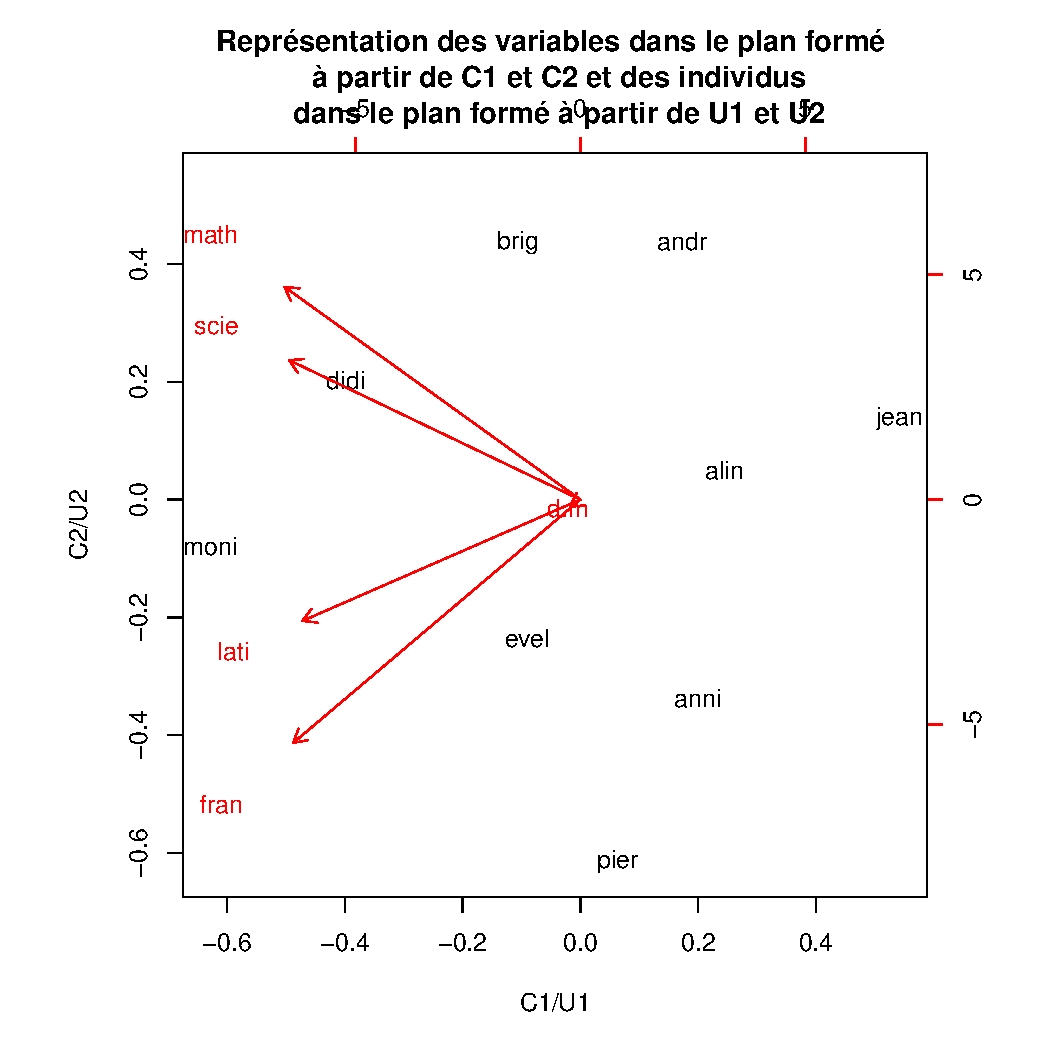
\includegraphics[width=0.35\textwidth]{22ex_base_et_individus_u1_u2.pdf}
    \captionof{figure}{Représentation des variables dans le plan formé à partir de C1 et C2 et des individus dans le plan formé à partir de U1 et U2}\label{fig:ana225}
\endgroup

\begingroup
    \centering
   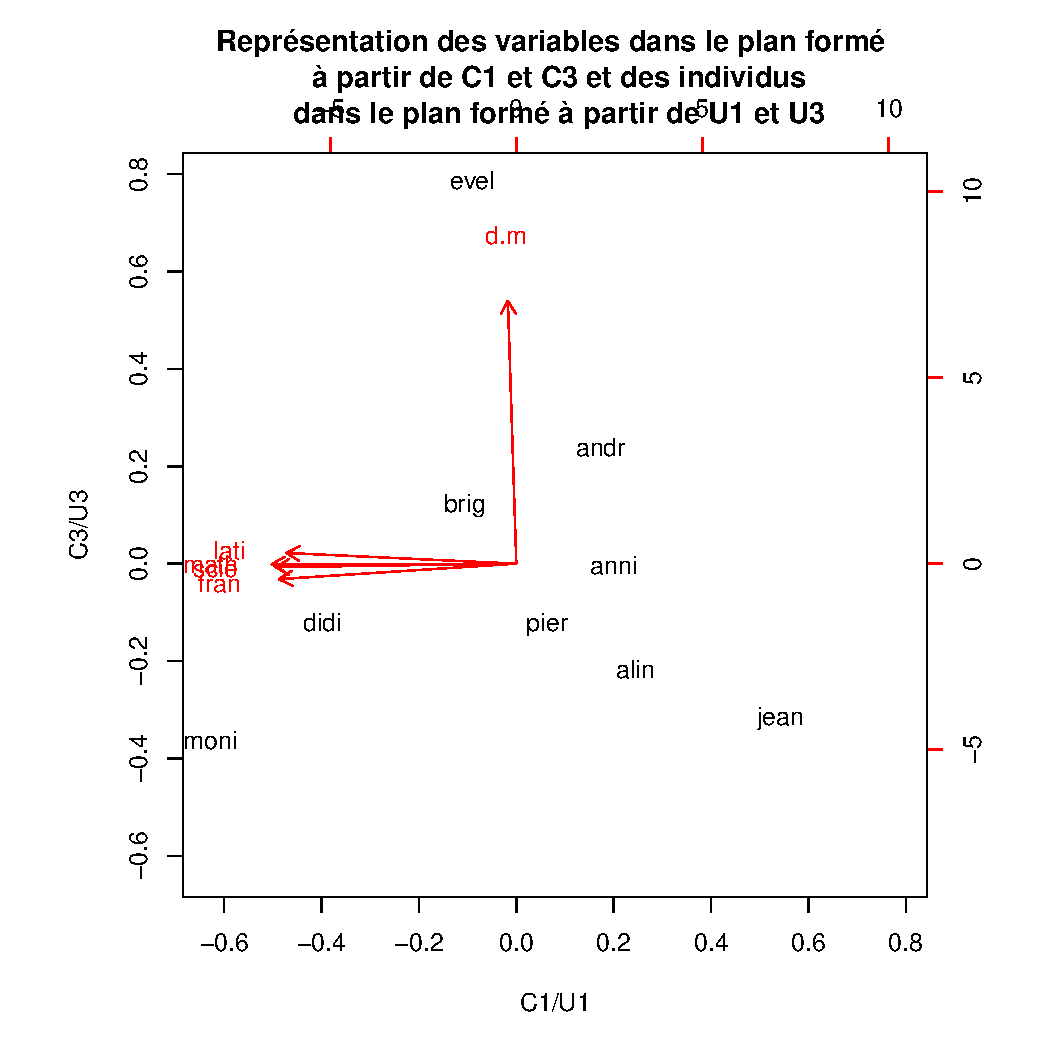
\includegraphics[width=0.35\textwidth]{22ex_base_et_individus_u1_u3.pdf}
    \captionof{figure}{Représentation des variables dans le plan formé à partir de C1 et C3 et des individus dans le plan formé à partir de U1 et U3}\label{fig:ana226}
\endgroup
\newpage
\subsection{Traitement des données Crabs}

On effectue l'\texttt{ACP} sur nos données \texttt{crabsquant} sans pré traitement pour le moment.

% \begin{multicols}{3} % Style triple colonne 

\begingroup
    \centering
   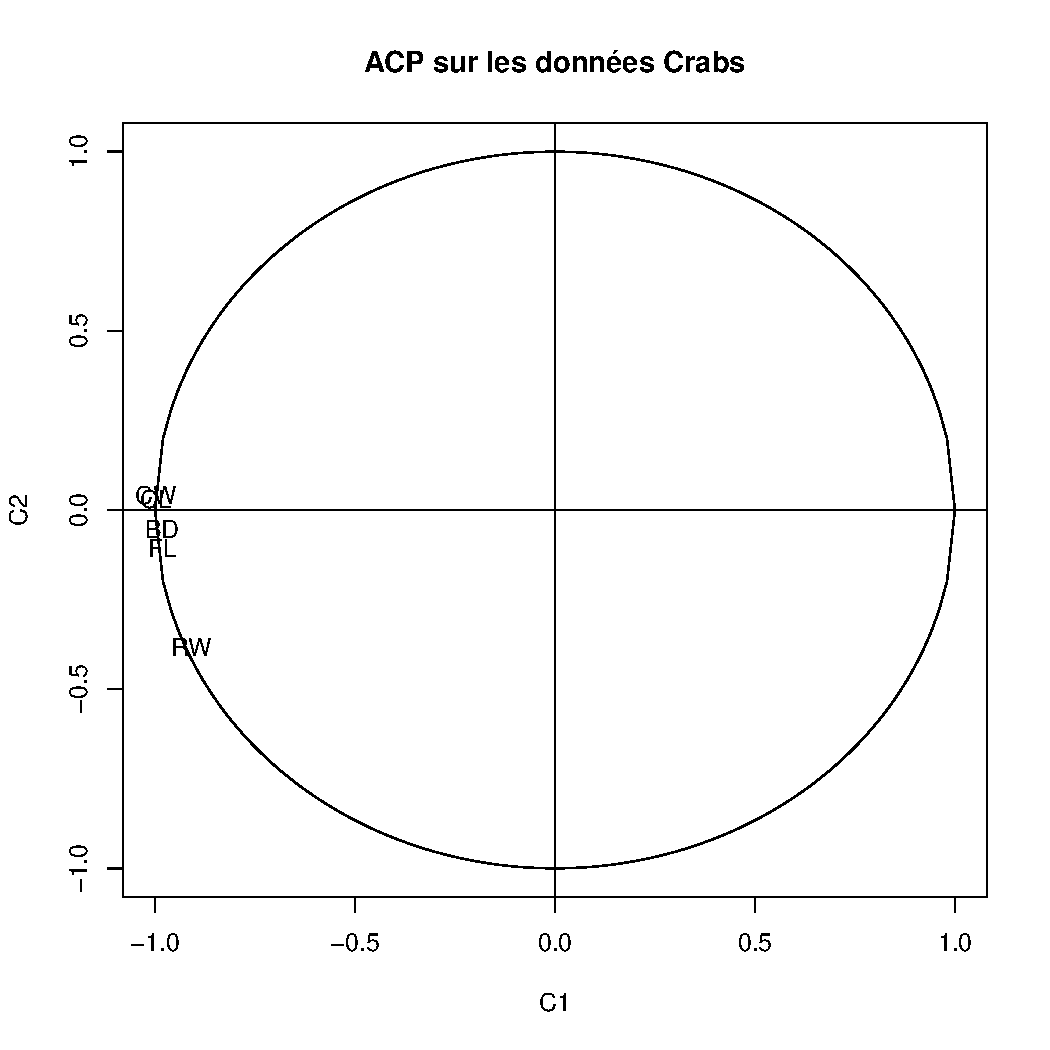
\includegraphics[width=0.35\textwidth]{variables_crabsc1c2.pdf}
    \captionof{figure}{Corrélation entre les variables des données Crabs et les composantes principales}\label{fig:crabs231}
\endgroup

\begingroup
    \centering
   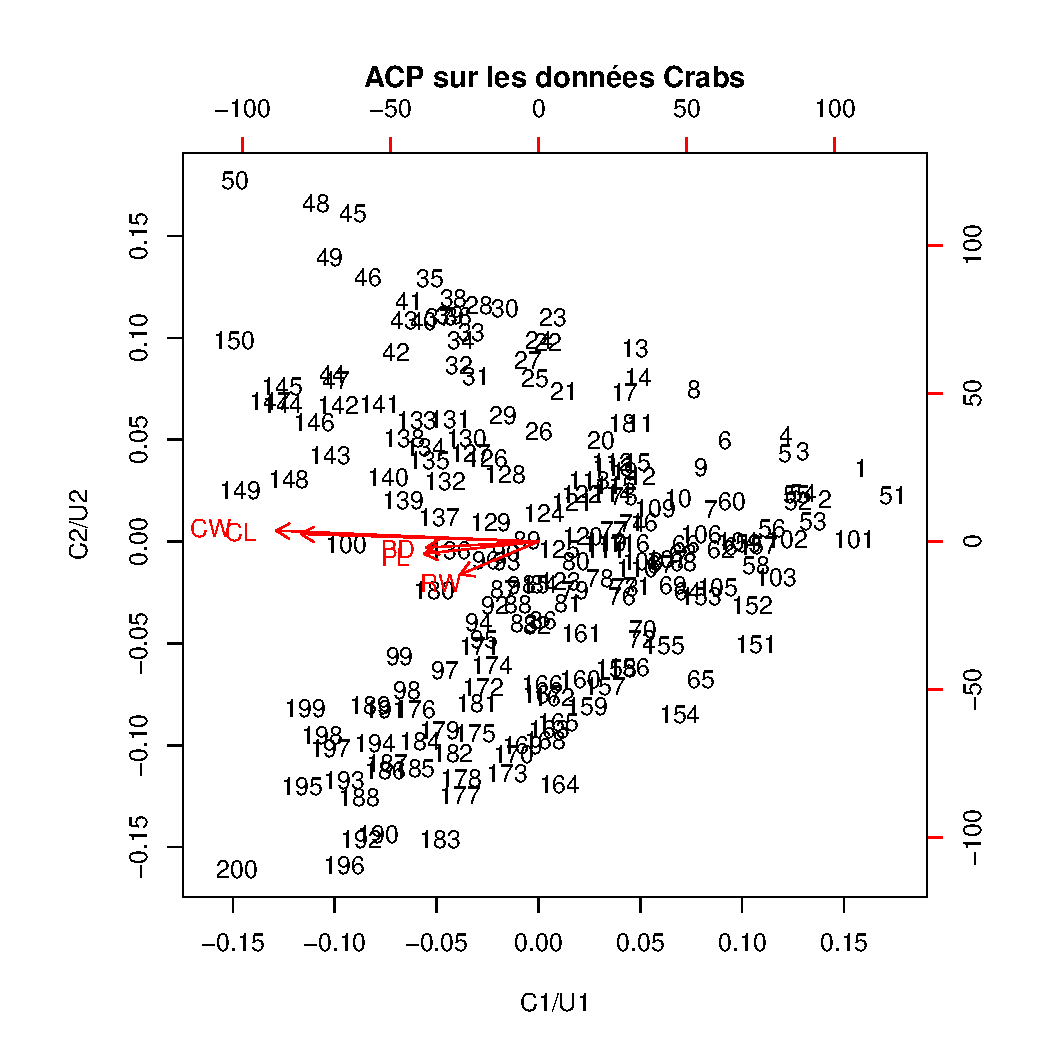
\includegraphics[width=0.35\textwidth]{ex_base_et_individus_u1_u2.pdf}
    \captionof{figure}{Plan de représentation des données Crabs}\label{fig:crabs232}
\endgroup

\begingroup
    \centering
   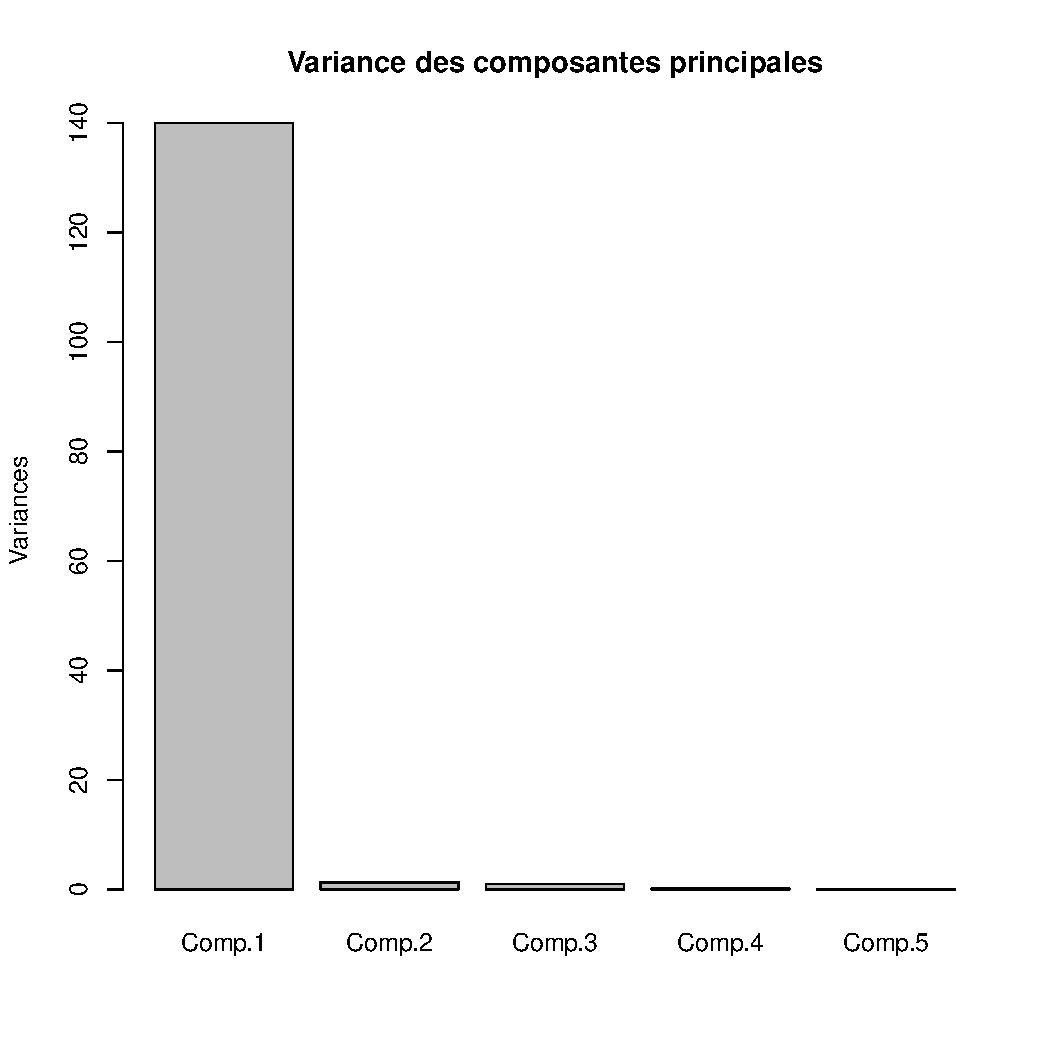
\includegraphics[width=0.35\textwidth]{batons_valeurs_propres.pdf}
    \captionof{figure}{Variance des composantes principales}\label{fig:crabs233}
\endgroup

% \end{multicols}

On observe dans les figures \ref{fig:crabs231} et \ref{fig:crabs232} que les variables sont très corrélées à la première composante principale et que la variance de la première composante (la première valeur propre) est très élevée. En appelant la fonction \textit{summary}, on constate que le pourcentage d'inertie expliquée par le premier axe est de $98 \%$. 

Ces résultats étaient particulièrement prévisibles. Effectivement, dans la sous section \ref{sub_sec_donnees_crabs}, nous avions stipulé qu'il y avait des relations linéaires entre chaque couple de variables quantitatives. Ainsi, le sous espace vectoriel $E_1 = \Delta u_1$ de dimension $1$ maximisant l'inertie expliquée par l'axe $\Delta u_1$ capture ces relations linéaires entre chaque couple de variables quantitatives. Par conséquent, la projection des individus sur $E_1$ devrait limiter la perte d'informations. 

Toutefois, afin d'améliorer notre représentation en termes de visualisation des différents groupes (les crabes mâles et bleu, les crabes mâles et orange, les crabes femelles et bleu ainsi que les crabes femelles et orange), on va donc pré traiter les données.

\begingroup
    \centering
   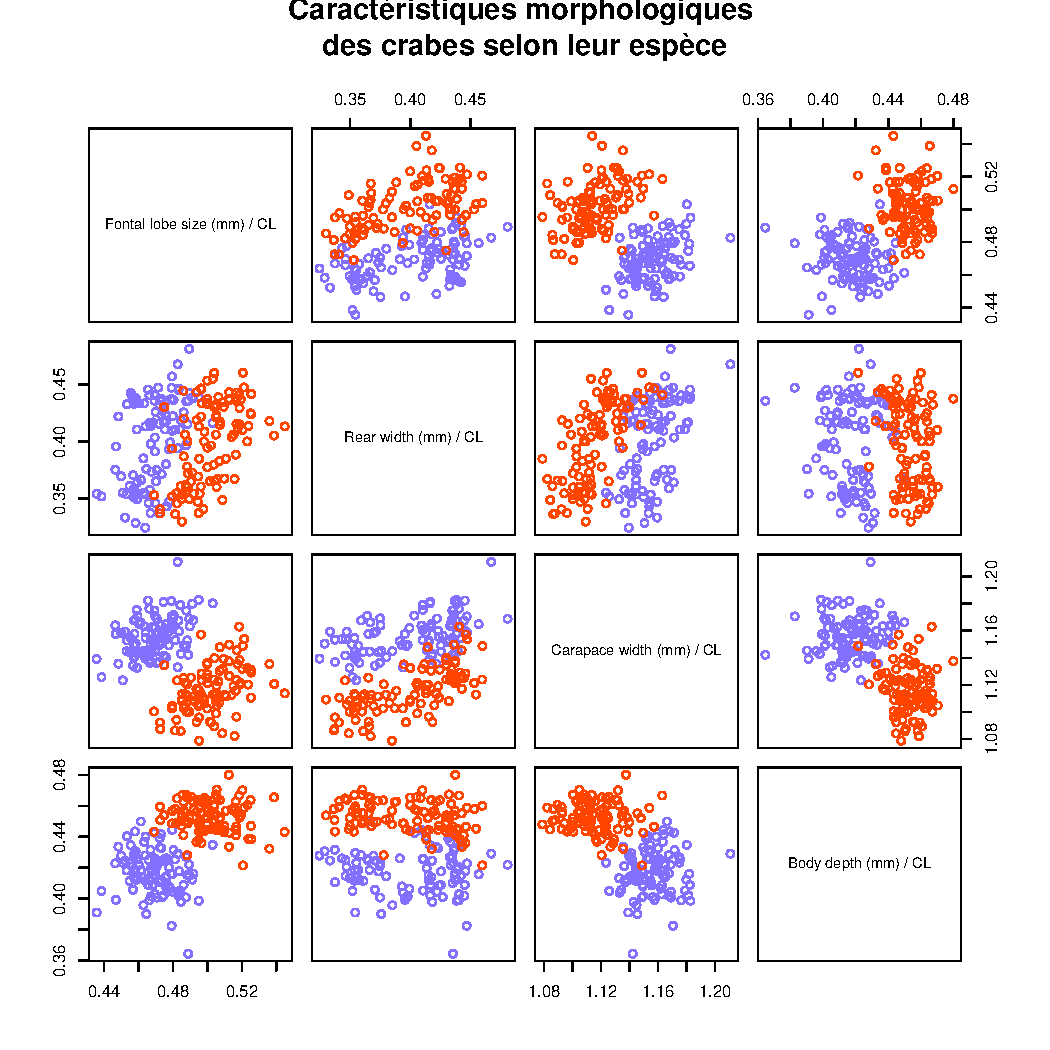
\includegraphics[width=0.35\textwidth]{PTcrabes_selon_espece.pdf}
    \captionof{figure}{Comparaison des caractéristiques morphologiques des crabes par espèce}\label{fig:crabs236}
\endgroup

\begingroup
    \centering
   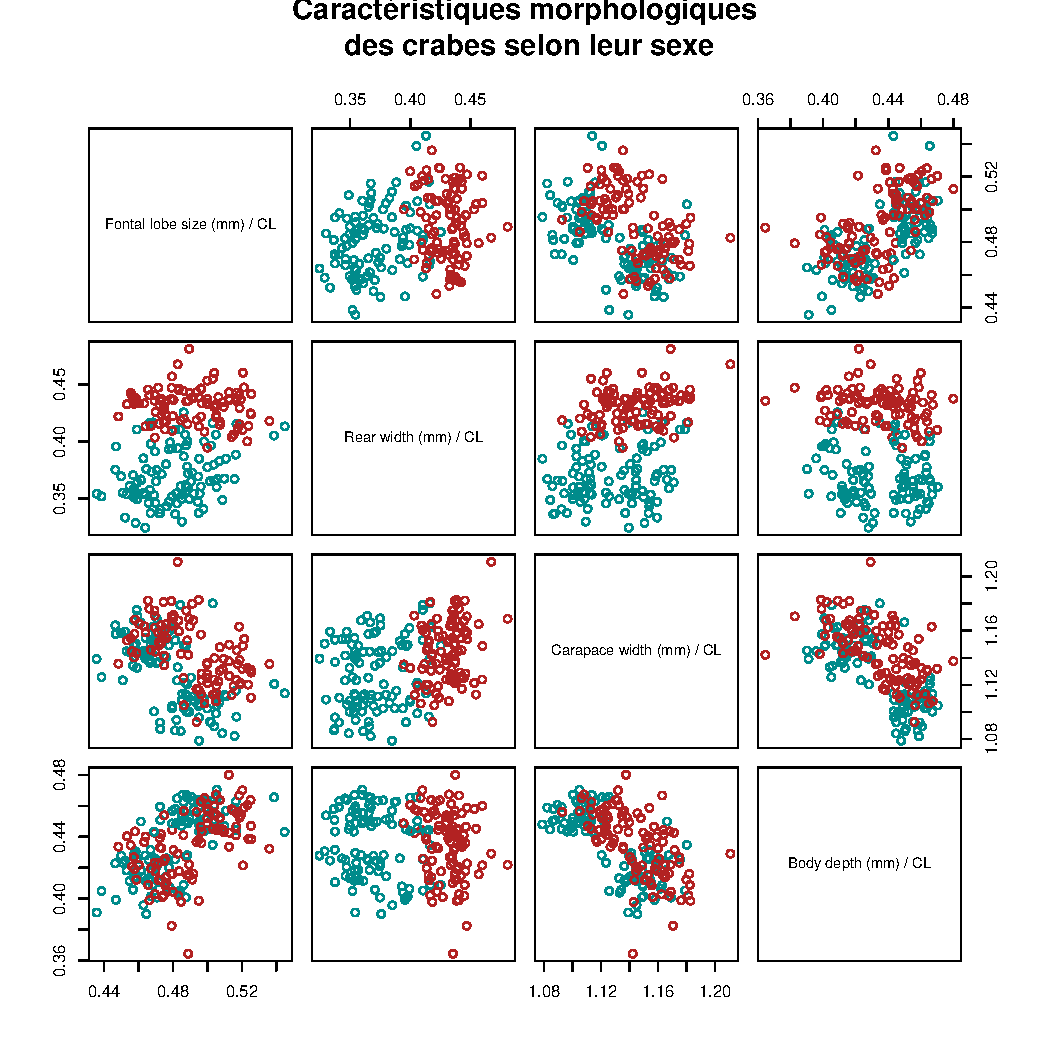
\includegraphics[width=0.35\textwidth]{PTcrabes_selon_sexe.pdf}
    \captionof{figure}{Comparaison des caractéristiques morphologiques des crabes par sexe}\label{fig:crabs237}
\endgroup

Dans les figures \ref{fig:crabs121} et \ref{fig:crabs122}, nous voyons que les lignes et les colonnes avec le paramètre \texttt{CL} nous permettent de dissocier les individus des différents groupes. Ainsi, nous suspectons que le rapport entre une variable autre que \texttt{CL} et le paramètre \texttt{CL} sont de "bons" indicateurs permettant de dissocier les individus. Dans les graphiques \ref{fig:crabs236} et \ref{fig:crabs237}, nos hypothèses sur les $4$ nouvelles variables sont confirmées.

En effectuant une \texttt{ACP} en se basant sur les quatre nouveaux indicateurs \texttt{FL/CL}, \texttt{RW/CL}, \texttt{CW/CL} et \texttt{BD/CL}, on obtient alors les résultats suivants. 

\begingroup
    \centering
   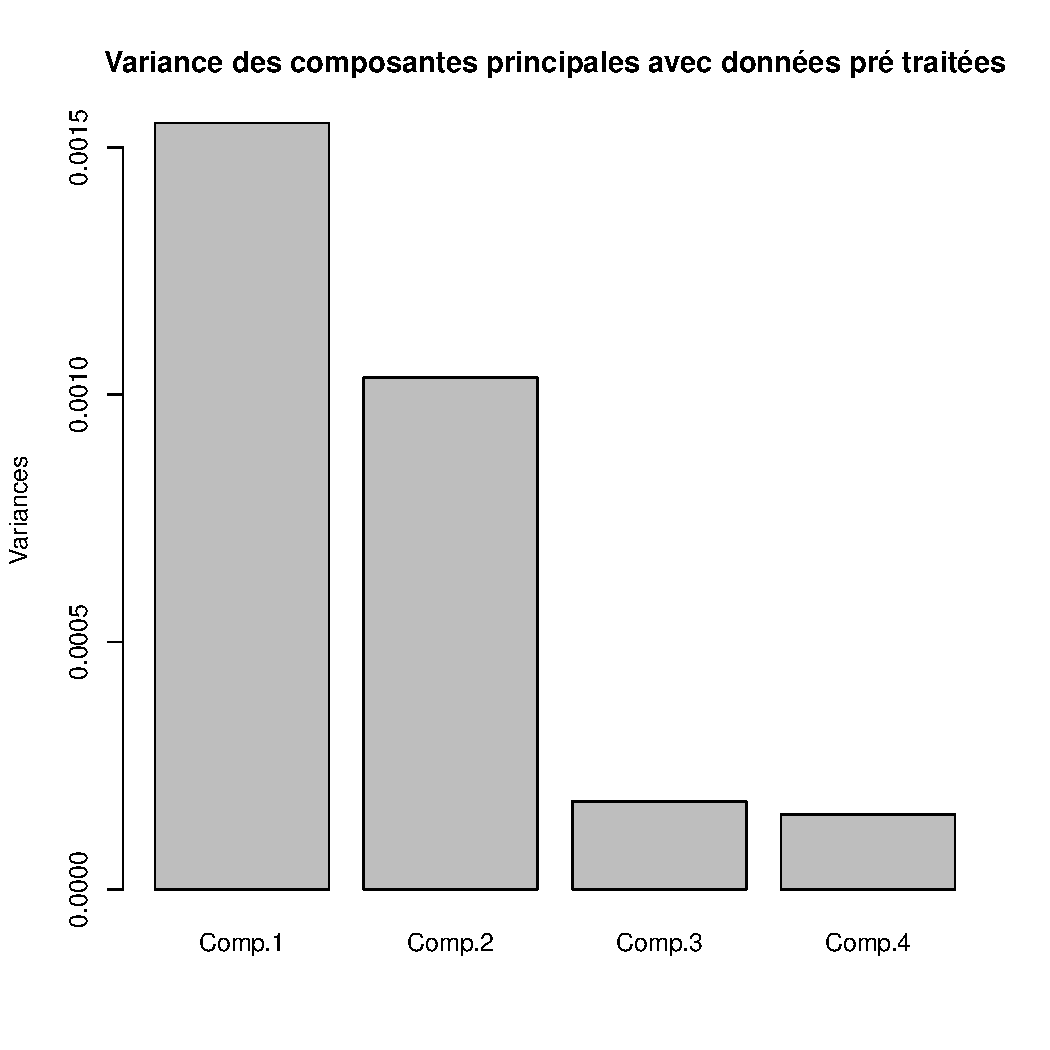
\includegraphics[width=0.35\textwidth]{PTbatons_valeurs_propres.pdf}
    \captionof{figure}{Variance des composantes principales}\label{fig:crabs235}
\endgroup

\begingroup
    \centering
   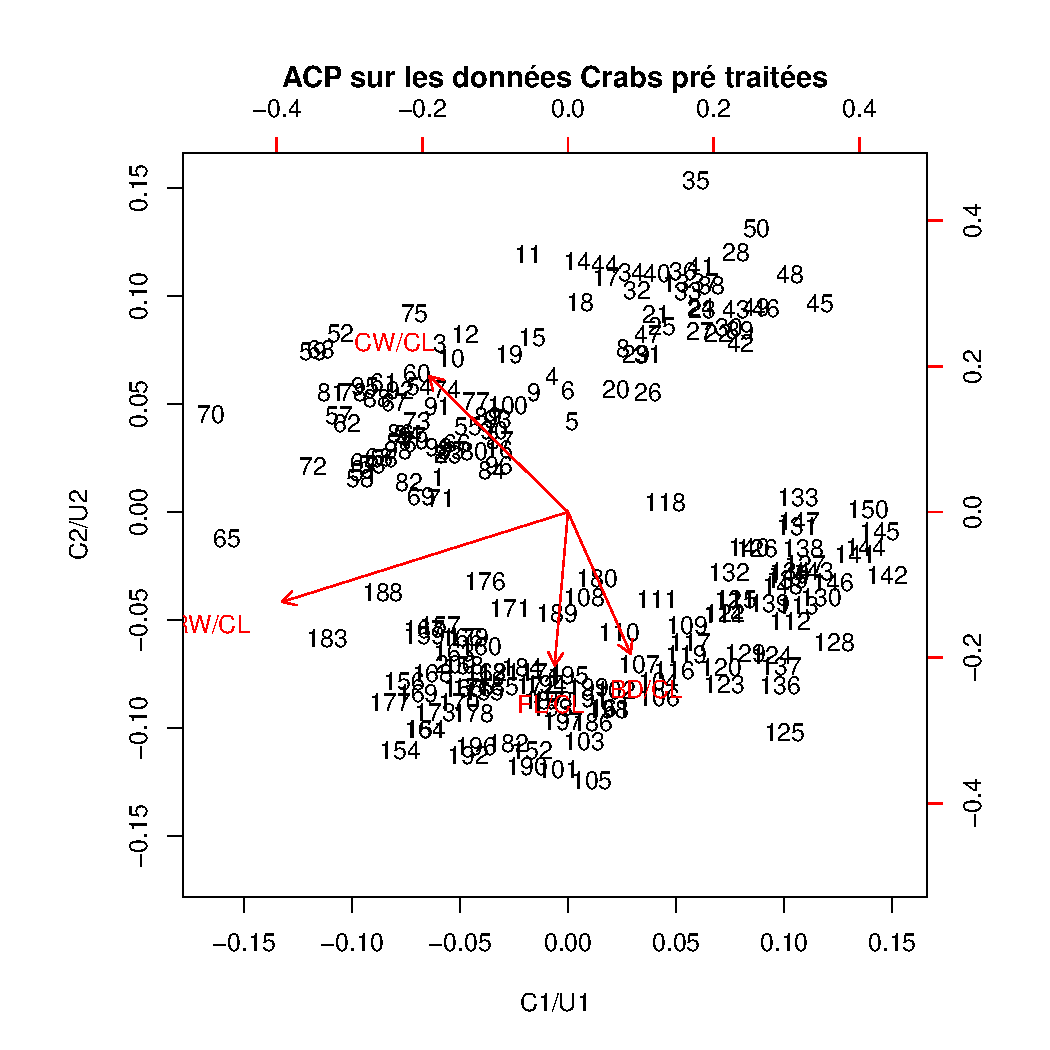
\includegraphics[width=0.35\textwidth]{PTex_base_et_individus_u1_u2.pdf}
    \captionof{figure}{Plan de représentation des données Crabs pré traitées (\texttt{FL/CL}, \texttt{RW/CL}, \texttt{CW/CL} et \texttt{BD/CL})}\label{fig:crabs234}
\endgroup

Dans la figure \ref{fig:crabs235}, on constate logiquement que le pourcentage d'inertie expliquée par le premier axe factoriel est plus faible que celui dans la figure \ref{fig:crabs233}.

Dans la figure \ref{fig:crabs234}, on constate que le premier axe factoriel traduit principalement les variables \texttt{BD/CL} et \texttt{FL/CL}. Le deuxième axe factoriel semble traduire la variable \texttt{RW/CL}. Ainsi, on peut émettre les observations suivantes :
\begin{itemize}
  \item un groupe a des rapports \texttt{BD/CL} et \texttt{FL/CL} relativement élevés mais un rapport \texttt{RW/CL} relativement bas 
  \item un groupe a des rapports \texttt{BD/CL} et \texttt{FL/CL} relativement élevés ainsi qu'un rapport \texttt{RW/CL} relativement élevé 
  \item un groupe a des rapports \texttt{BD/CL} et \texttt{FL/CL} relativement bas mais un rapport \texttt{RW/CL} relativement élevé 
  \item un groupe a des rapports \texttt{BD/CL} et \texttt{FL/CL} relativement bas ainsi qu'un rapport \texttt{RW/CL} relativement bas 
\end{itemize}

\section{Conclusion}

En conclusion, au cours de ce rapport, nous avons pu utiliser de façon concrète la puissance et les multiples possibilités qui s’offrent à nous en terme de traitement statistique de données avec \texttt{R}. Grâce à la statistique descriptive, nous avons appris à faire ressortir les données qui nous intéressent à travers un large jeu. Nous avons ensuite appliqué la méthode de l’\texttt{ACP} qui nous a considérablement aidés à obtenir des données analysables sous un plan qui ne s’offrait pas directement à nous d'un premier abord.

\end{multicols}

\end{document}